%2multibyte Version: 5.50.0.2953 CodePage: 65001
% Asian Technology Conference in Mathematics (ATCM) %
% style sheet for LaTeX.  Please do not modify sections   %
% or commands marked 'eJMT'.                              %
% eJMT commands                                           %
% see note below            %
% ATCM page dimensions                                    %
% ATCM header & footer                                    %
% Please place your own definitions here
% How to use hyperref                                     %
% -------------------                                     %
% Probably the only way you will need to use the hyperref %
% package is as follows.  To make some text, say          %
% "My Text Link", into a link to the URL                  %
% http://something.somewhere.com/mystuff, use             %
% \href{http://something.somewhere.com/mystuff}{My Text Link}

\documentclass[12pt,a4paper]{article}%
\usepackage{amsfonts}
\usepackage{amsmath}
\usepackage[a4paper]{geometry}
\usepackage{fancyhdr}
\usepackage{amssymb}
\usepackage{color}
\usepackage[pdftex]{hyperref}
\usepackage{graphicx}
\usepackage{subfigure}%
\setcounter{MaxMatrixCols}{30}
%TCIDATA{OutputFilter=latex2.dll}
%TCIDATA{Version=5.50.0.2953}
%TCIDATA{Codepage=65001}
%TCIDATA{LastRevised=Thursday, December 20, 2018 20:23:38}
%TCIDATA{<META NAME="GraphicsSave" CONTENT="32">}
%TCIDATA{<META NAME="SaveForMode" CONTENT="1">}
%TCIDATA{BibliographyScheme=Manual}
%TCIDATA{Language=American English}
%BeginMSIPreambleData
\providecommand{\U}[1]{\protect\rule{.1in}{.1in}}
%EndMSIPreambleData
\hypersetup{                                                  a4paper,                                                  breaklinks                                            }
\newtheorem{theorem}{Theorem}
\newtheorem{acknowledgement}[theorem]{Acknowledgement}
\newtheorem{algorithm}[theorem]{Algorithm}
\newtheorem{axiom}[theorem]{Axiom}
\newtheorem{case}[theorem]{Case}
\newtheorem{claim}[theorem]{Claim}
\newtheorem{conclusion}[theorem]{Conclusion}
\newtheorem{condition}[theorem]{Condition}
\newtheorem{conjecture}[theorem]{Conjecture}
\newtheorem{corollary}[theorem]{Corollary}
\newtheorem{criterion}[theorem]{Criterion}
\newtheorem{definition}[theorem]{Definition}
\newtheorem{example}[theorem]{Example}
\newtheorem{exercise}[theorem]{Exercise}
\newtheorem{lemma}[theorem]{Lemma}
\newtheorem{notation}[theorem]{Notation}
\newtheorem{problem}[theorem]{Problem}
\newtheorem{proposition}[theorem]{Proposition}
\newtheorem{remark}[theorem]{Remark}
\newtheorem{solution}[theorem]{Solution}
\newtheorem{summary}[theorem]{Summary}
\newenvironment{proof}[1][Proof]{\noindent\textbf{#1.} }  {\ \rule{0.5em}{0.5em}}
\pagestyle{empty}
\setlength{\headheight}{14pt}
\geometry{left=2cm,right=2cm,top=3.2cm,bottom=3.2cm}
\pagestyle{fancyplain}
\fancyhf{}
\renewcommand{\headrulewidth}{0pt}

% Local definitions

\graphicspath{{./Images_Meade/}}

\begin{document}

\title{\textbf{Locus Problems Related to Linear Combinations of Vectors}}

\author{\textit{Wei-Chi YANG}\\wyang@radford.edu\\Department of Mathematics \\and Statistics\\Radford University\\Radford, VA 24142\\USA
\and
\textit{Douglas B. MEADE}\\meade@math.sc.edu\\Department of Mathematics\\University of South Carolina\\Columbia, SC 29208\\USA}
\date{}
\maketitle

\begin{abstract}
This paper is a more in-depth discussions for selected problems discussed in
\cite{ATCM2018}, which are inspired by college entrance exam practice problems
from China. When initially seeing the problem during an
exam, one may have no clue how the problem is created. In this paper, we
begin by presenting the essential algebraic manipulation skills that
Chinese high school students are expected to apply to answer the question.
We then continue the discussion by exploring
various scenarios that utilize technological tools. We shall
see many unexpected surprising outcomes. More importantly, we summarize how a
problem can be extended to a more general setting whenever is possible.

\end{abstract}
%document title

%Single author.  Please supply at least your name,
%email address, and affiliation here.

%
%%%%%%%%%%%%%%%%%%%%%%%%%%%%%%%%%%%%%%%%%%%%%%%%%%%%%%%%%%%
%%
%ATCM commands - do not change these                     %
%%

%%
%%%%%%%%%%%%%%%%%%%%%%%%%%%%%%%%%%%%%%%%%%%%%%%%%%%%%%%%%%%
%abstract

%
%%%%%%%%%%%%%%%%%%%%%%%%%%%%%%%%%%%%%%%%%%%%%%%%%%%%%%%%%%%
%%
%ATCM command                                            %
%%
\thispagestyle{fancy}
%%
%%%%%%%%%%%%%%%%%%%%%%%%%%%%%%%%%%%%%%%%%%%%%%%%%%%%%%%%%%%
%Please use the following to indicate sections, subsections,
%etc.  Please also use \subsubsection{...}, \paragraph{...}
%and \subparagraph{...} as necessary.


\section{Introduction} \label{sec1}

This paper is a more in depth discussion on selected problems from the
published article \cite{ATCM2018}. Finding a curve defined by the locus of a
moving point has been popular and such problems are often asked on Gaokao (a college entrance
exam) in China. There have been several exploratory activities (see
\cite{June2017} \cite{MacandYang}, and \cite{YangandS}) derived from Chinese
college entrance exam practice problems (see \cite{Gao}). In this article, we
typically start with a practice problem originated from (\cite{Gao}) to
initiate our discussions. We demonstrate how a problem can be solved without
the assistance of technological tools, which shall demonstrate those crucial
algebraic manipulation skills that are required by high school students from
China. From a content knowledge point of view, this paper is very accessible to
those students who have learned parametric equations and have a basic understaning of
linear algebra. Problems presented in this paper can be used as examples for
professional training purposes.

In this paper, we stress that if problems are presented as explorations instead
of in an examination setting, learners would enjoy learning some new mathematics
more than simply performing a collection of somewhat boring algebraic manipulations.
We believe making
conjectures by seeing possible solutions before asking complete analytic or
algebraic solutions is much more accessible, convincing and intuitive to
students. In addition to solving simple cases by hand, we typically construct
a potential solution geometrically using the trace feature of dynamic geometry
software (DGS) such as Geometry Expressions \cite{GE}.
Finally, we use a computer algebra system (CAS) such as Maple \cite{Maple}
to verify that our analytic solutions are identical to those obtained by using the DGS.

\section{Locus from Shifting and Scaling} \label{sec2}

In the first set of problems we consider we are given two fixed points
and a moving point on a smooth convex
curve, and need to find the locus of a point lying on the line segment
connecting one fixed point and a moving point. We first present the original
problem and solve it by hand and then see how the problem can be extended to
other scenarios in 2D. Next, we summarize how the problem is related to the
translation and scaling of figures.

\subsection{Generating a circle with two fixed points} \label{ssec2-1}

The setting for our first locus problem has a fixed point on a circle and another
fixed point that is not on the circle. 
Example~\ref{ex1} is a slightly modified version of the original practice problem discussed
in the Introduction
(see \cite{Gao}).

\begin{example} \label{ex1}
In Figure~\ref{fig1} we are given a fixed circle in blue,
$(x-a)^{2}+(y-b)^{2}=r^{2}$ and the moving point $D=(x_{0},y_{0})$
is on the circle. Furthermore we choose the fixed point $C=(c,d)$ that is
not on the circle and let $E$ be the midpoint of $CD$.
The goal is to find the locus of $E$.%
\begin{figure}[htbp]
\begin{center}
 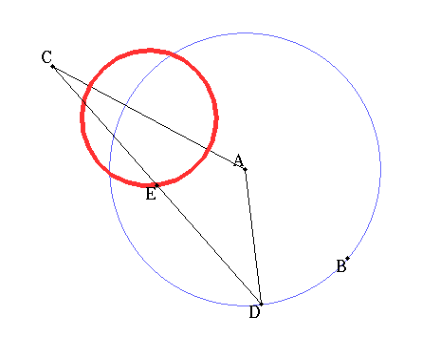
\includegraphics[width=2.0in,keepaspectratio]{PJH75H11-crop.pdf}
\end{center}
 \caption{Circle and two fixed points.}
 \label{fig1}
\end{figure}
\end{example}

We first see how students solve this problem by hand in an exam. We note that
the midpoint $E$ of $CD$ can be written as
$E=\left(  \frac{c+x_{0}}{2}, \frac{d+y_{0}}{2}\right)$.
Let $x=\frac{c+x_{0}}{2}$ and $y=\frac{d+y_{0}}{2}$.
Then we see $\left(  \left(  2x-c\right)  -a\right)  ^{2}+\left(\left(  2y-d\right)  -b\right)  ^{2}=r^{2}$,
which implies that
\begin{align*}
\left(  2x-c\right)  ^{2}-2a\left(  2x-c\right)  +a^{2}+\left(  2y-d\right)
^{2}-2b\left(  2y-d\right)  +b^{2}  & =r^{2}\\
4x^{2}-4cx+c^{2}-4ax+2ac+a^{2}+4y^{2}-4dy+d^{2}-4by+2bd+b^{2}  & =r^{2}%
\end{align*}
After simplifying, we see
\[
\left(  x-\left(  \frac{a+c}{2}\right)  \right)  ^{2}+\left(  y-\left(
\frac{b+d}{2}\right)  \right)  ^{2}=\frac{1}{4}r^{2}.
\]
Indeed the locus of the point $E$ is the circle with center $\left(  \frac{a+c}{2},\frac{b+d}{2}\right)$
and radius $\frac{r}{2}$.

\textbf{Exploration.} Following the discussions from Example~\ref{ex1}, if we let the
point $E$ satisfy $\overrightarrow{CE}=s\overrightarrow{CD}$ with
$s\in\left(  0,1\right)  $ and we would like to find the locus of $E,$ then it
is easy to verify that the locus for $E$ will be as follows:%
\[
\left(  x-s^{2}\left(  a+c\right)  \right)  ^{2}+\left(  y-s^{2}\left(
b+d\right)  \right)  ^{2}=\left(  sr\right)  ^{2}.
\]
To 

\subsection{Locus as a result of simple translation and scaling} \label{ssec2-2}

We may view the discussions in the preceding Example~\ref{ex1} as a simple
translation and scaling from a given curve to the other. For instance, if we
consider the given fixed points $C=$ $(c,d),A=(a,b)$ and a curve $C_{1}$ . We
assume $C\neq A.$ By taking the moving point $D$ to be on the curve $C_{1} $,
our objective is to find the locus of the midpoint $E$ of $CD.$ If $O$ denotes
the origin $(0,0),$then the locus $\overrightarrow{OE}=\overrightarrow
{OC}+\overrightarrow{CE}=\overrightarrow{OC}+\frac{1}{2}\overrightarrow{CD}.$
In particular, if $C_{1}$ represents the circle centered at $A$ and of radius
$r$, then the locus of the point $E$ will be the circle centered at $C$ and the radius is
being scaled to $\frac{1}{2}$ of the original circle. (See Figure~\ref{fig2}(a).) It is
clear now that if we were to find the locus of the point $E$ satisfying
$\overrightarrow{CE}=s\overrightarrow{CD}$, where $s\in[0,1]$, it is
equivalent to asking the locus of $\overrightarrow{OE}=\overrightarrow
{OC}+\overrightarrow{CE}=\overrightarrow{OC}+s\overrightarrow{CD},$ where
$s\in[0,1]$. If the equation of $C_{1}$ is represented by
$\left[
\begin{array}
[c]{c}%
x_{1}(t)\\
y_{1}(t)
\end{array}
\right]$, then we can write the locus of $\overrightarrow{OE}$ as
\begin{align*}
\left[
\begin{array}
[c]{c}%
x_{2}(t)\\
y_{2}(t)
\end{array}
\right]   & =\left[
\begin{array}
[c]{c}%
c\\
d
\end{array}
\right]  +s\left[
\begin{array}
[c]{c}%
x_{1}(t)-c\\
y_{1}(t)-d
\end{array}
\right] \\
& =(1-s)\left[
\begin{array}
[c]{c}%
c\\
d
\end{array}
\right]  +s\left[
\begin{array}
[c]{c}%
x_{1}(t)\\
y_{1}(t)
\end{array}
\right]  .
\end{align*}
If $C_{1}$ represents the circle centered at $A$ and of radius $r,$ the locus
of $\overrightarrow{OE}$ can be viewed as a result of the combination of
translation and scaling. Figure~\ref{fig2}(b) shows the translation and scaling
when $s=\frac{1}{4}$.

It is clear that there can be more than one way of expressing the locus of $E$.
For example, we may write $\overrightarrow{OE}=\overrightarrow{OA}%
+\overrightarrow{AE}=\overrightarrow{OA}+\overrightarrow{AC}+\overrightarrow
{CE}=\overrightarrow{OA}+\overrightarrow{AC}+\frac{1}{2}\overrightarrow
{CD}=\overrightarrow{OA}+\overrightarrow{AC}+$ $\frac{1}{2}\left(
\overrightarrow{AD}-\overrightarrow{AC}\right)  =\overrightarrow{OA}+\frac
{1}{2}\left(  \overrightarrow{AC}+\overrightarrow{AD}\right)  $. To find the
locus of the point $F$ satisfying $\overrightarrow{CF}=s\overrightarrow{CD},$
where $s\in(0,1)$, in this case, we note $\overrightarrow{OF}=\overrightarrow
{OA}+\overrightarrow{AF},$ where
\begin{align}
\overrightarrow{AF}  & =\overrightarrow{AC}+s\overrightarrow{CD}\label{eq9b}\\
& =\overrightarrow{AC}+s\left(  \overrightarrow{AD}-\overrightarrow{AC}\right)
\nonumber\\
& = \left(  1-s\right) \overrightarrow{AC}  + s \overrightarrow{AD},
\end{align}
If the equation of $C_{1}$ is represented by $\left[
\begin{array}
[c]{c}%
x_{1}(t)\\
y_{1}(t)
\end{array}
\right]$, then the locus of $\overrightarrow{OE}$ can be written as
\[
\left[
\begin{array}
[c]{c}%
x_{2}(t)\\
y_{2}(t)
\end{array}
\right]  =\left[
\begin{array}
[c]{c}%
a\\
b
\end{array}
\right]  +(1-s)\left[
\begin{array}
[c]{c}%
c-a\\
d-b
\end{array}
\right]  +s\left[
\begin{array}
[c]{c}%
x_{1}(t)-a\\
y_{1}(t)-b
\end{array}
\right],
\]
where $s\in[0,1]$. We see that when $s=0$ we get the point $C$ and
when $s=1$ we get the parametric curve $C_{1}$. In particular,
Figure~\ref{fig2}(b) shows the translation and scaling when $s=\frac{1}{4}$ and $C_{1}$ is a
circle.

\begin{figure}[htpb]
\begin{center}
\parbox[b]{1.7in}{\begin{center}
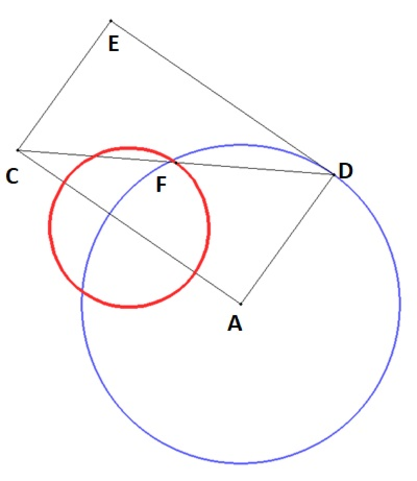
\includegraphics[width=1.7in,keepaspectratio]{Figure6-crop.pdf}
 \\ (a)
\end{center}}
\qquad
\parbox[b]{1.7in}{\begin{center}
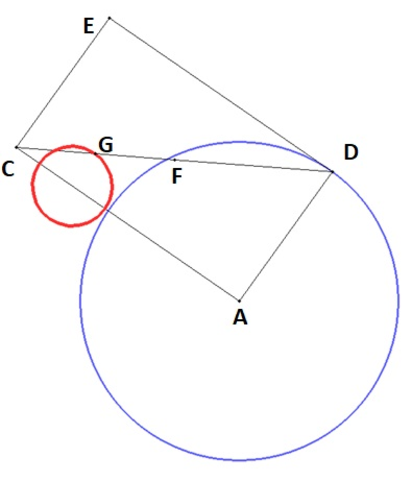
\includegraphics[width=1.7in,keepaspectratio]{Figure7-crop.pdf}
 \\ (b)
\end{center}}
\end{center}
\caption{Locus of the point $F$ (a) when $s=\frac{1}{2}$ and (b) when $s=\frac{1}{4}$.}
\label{fig2}
\end{figure}

Analytic verification that the locus is a simple translation and scaling
is easily completed with the help of a CAS such as Maple \cite{Maple}.
Figure~\ref{fig3} shows six snapshots of the translation and scaling
for the case when $A=(a,b)=(-.725,.15),r=.7685864$, and $C=(c,d)=(-1.8,0.89)$.
In each frame the locus is a circle centered at a point lying along
the line segment $AC$ (because of the factor $(1-s) \overrightarrow{AC}$
in \ref{eq9b}) and
each radius increases as $s$ increases (due to the
factor of $s \overrightarrow{AD}$ in \ref{eq9b}).

\begin{figure}
\begin{center}
\parbox[b]{1.5in}{\begin{center}
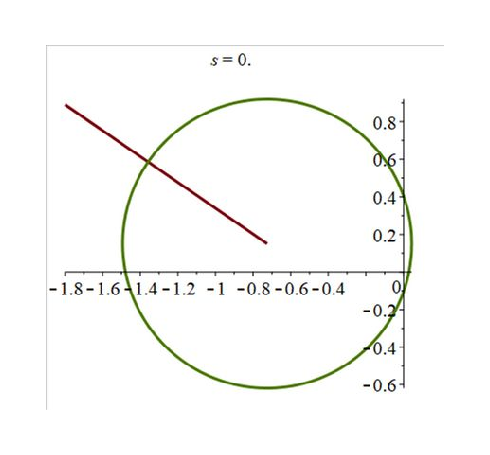
\includegraphics[width=1.5in,trim=0mm 0mm 0mm 15mm,clip,keepaspectratio]{PJH75H12.pdf}
\\
(a)
\end{center}}
\qquad
\parbox[b]{1.5in}{\begin{center}
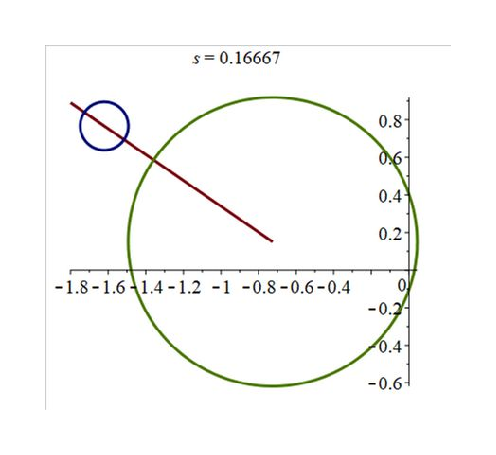
\includegraphics[width=1.5in,trim=0mm 0mm 0mm 15mm,clip,keepaspectratio]{PJH75H13.pdf}
\\
(b)
\end{center}}
\qquad
\parbox[b]{1.5in}{\begin{center}
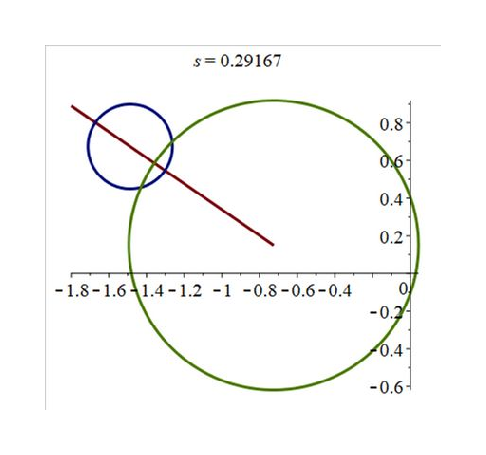
\includegraphics[width=1.5in,trim=0mm 0mm 0mm 15mm,clip,keepaspectratio]{PJH75H14.pdf}
\\
(c)
\end{center}}
\\
\parbox[b]{1.5in}{\begin{center}
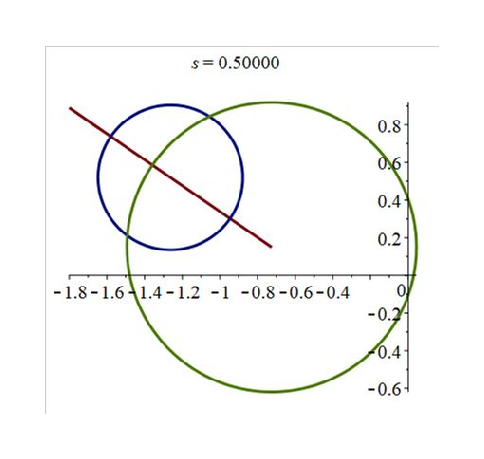
\includegraphics[width=1.5in,trim=0mm 0mm 0mm 15mm,clip,keepaspectratio]{PJH75H15.pdf}
\\
(d)
\end{center}}
\qquad
\parbox[b]{1.5in}{\begin{center}
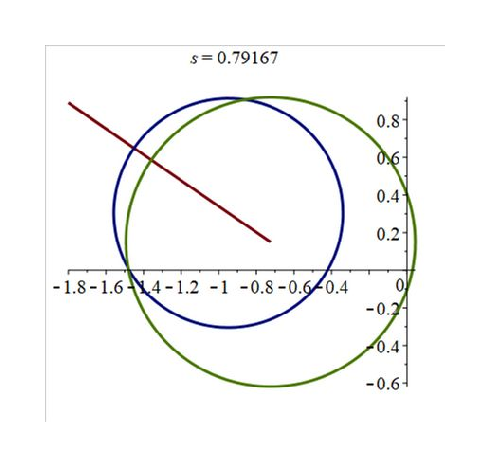
\includegraphics[width=1.5in,trim=0mm 0mm 0mm 15mm,clip,keepaspectratio]{PJH75H16.pdf}
\\
(e)
\end{center}}
\qquad
\parbox[b]{1.5in}{\begin{center}
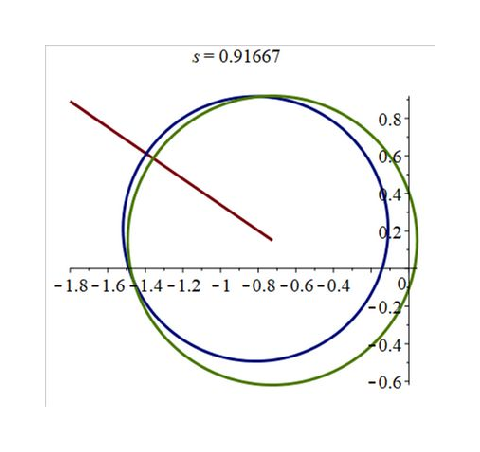
\includegraphics[width=1.5in,trim=0mm 0mm 0mm 15mm,clip,keepaspectratio]{PJH75H17.pdf}
\\
(f)
\end{center}}
\end{center}
\caption{Locus of the point $E$
               (a) when $s=0$, (b) when $s=0.16667$, (c) when  $s=0.29167$,
               (d) when $s=0.5$, (e) when $s=0.79167$, and (f) when $s=0.91667$.}
\label{fig3}
\end{figure}

Supplemental resource [S1] provides a framework for further hands-on
exploration on this problem and other interesting translation and scaling
problems. In particular, we encourage readers to explore this problem
when the circle is replaced with an ellipse as follows:

\begin{exercise} \label{ex2}
Suppose we are given an ellipse and two fixed points $A$ and $C$ respectively
where $A$ is the center of the ellipse and $C\neq A$. (See Figure~\ref{fig4}.)
 We let $D$ be a moving point on the ellipse and $E$ be a point such that
$\overrightarrow{CE}=s\overrightarrow{CD},$ $s\in[0,1]$.
Find the locus $\overrightarrow{OE}=\overrightarrow{OA}+\overrightarrow{AE}$.
\end{exercise}

It is clear that the locus in this case is a result of simple translation and
scaling from the original ellipse. The two scenarios in Figure~\ref{fig4}
show the locus $\overrightarrow{OE}$ in red when $s=\frac{1}{2}$ and
$\frac{1}{4}$ respectively.
Here we use the ellipse of $\frac{x^{2}}{4}+y^{1}=1$ and the fixed point $C=[0,1.3]$.

\begin{figure}[htpb]
\begin{center}
\parbox[b]{2.2in}{\begin{center}
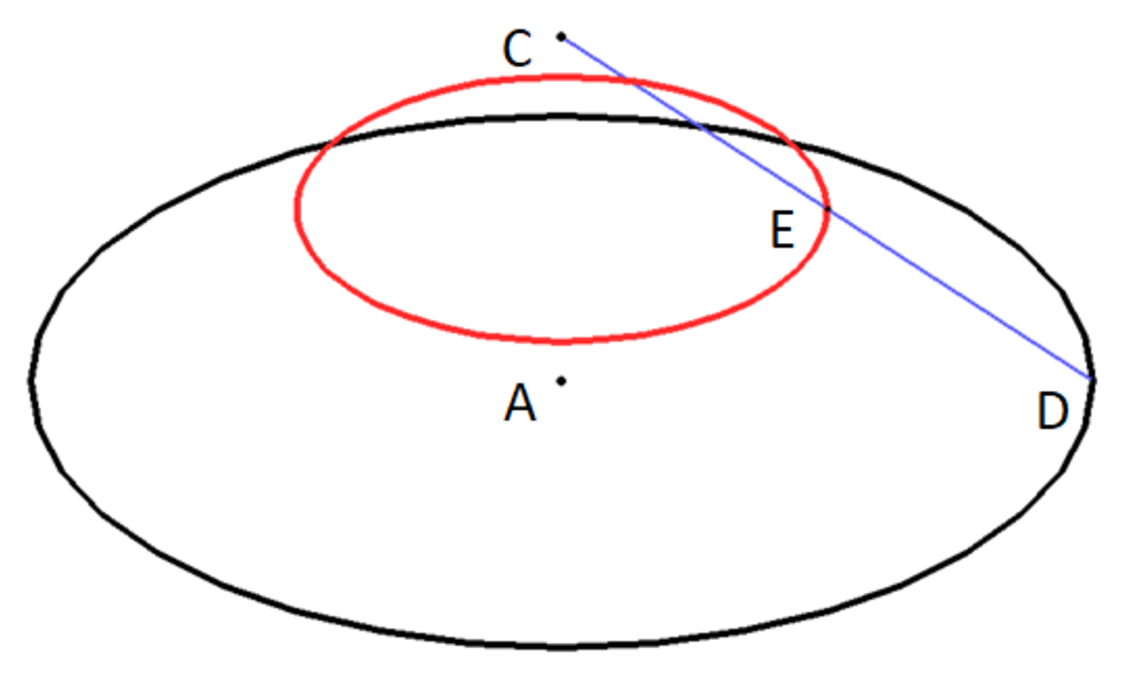
\includegraphics[width=2.2in,keepaspectratio]{exercise2-crop.pdf}
 \\ (a)
\end{center}}
\qquad
\parbox[b]{2.2in}{\begin{center}
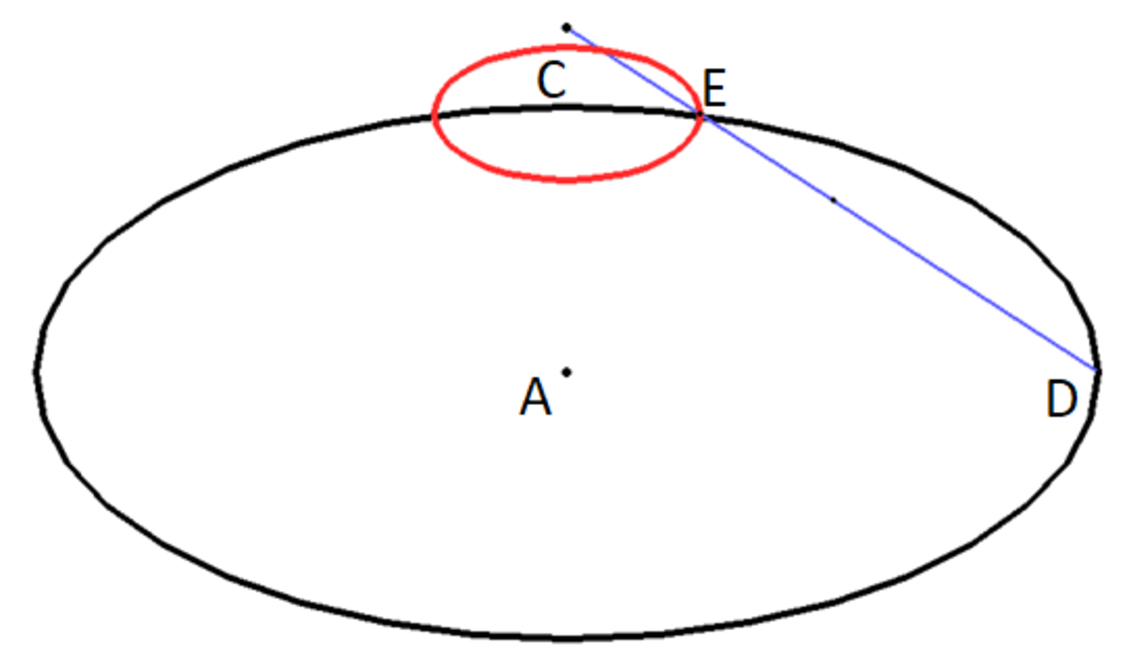
\includegraphics[width=2.2in,keepaspectratio]{exercise2(b)-crop.pdf}
 \\ (b)
\end{center}}
\end{center}
\caption{Snapshots from the transition between two ellipses when (a) $s=\frac{1}{2}$ and (b) $s=\frac{1}{4}$.}
\label{fig4}
\end{figure}

The following observation is a simple result of \ref{eq9b}. More exploration
can be found in supplemental resource [S1].

\begin{theorem}
Let $A=\left(  a,b\right)$, $C=(c,d)$ be two fixed points and $P$ represent a
closed parametric curve that is represented by
$[x(a,b,r,t), y(a,b,r,t)] = [a+f(r,t)\cos t, b+g(r,t)\sin t]$ where $f(r,0)=0$
and $t\in[0, 2\pi]$. If $D$ is a moving point on $P$, then the locus $F$
satisfying $\overrightarrow{CF}=s\overrightarrow{CD}$, $s\in[0,1]$, is a
simple translation of the parametric curve from point $C$ to point $A$ with a
scaling factor of $s$. In particular, when $f(r,t)$ and $g(r,t)$ are positive constants
then $P$ is an ellipse and the locus corresponds to a translation and scaling of this ellipse.
\end{theorem}

In higher dimensions there can be more than one way of expressing the locus for the translation
and scaling. We describe our 3D extension as follows:

\begin{theorem}
Let $A=(a, b, c )$, $C=(d,e,f)$ be two fixed points and $P$ represent
a closed parametric surface that is represented by $\overrightarrow
{OA}+\left[
\begin{array}
[c]{c}%
x_{1}(t_{1},t_{2})\\
y_{1}(t_{1},t_{2})\\
z_{1}(t_{1},t_{2})
\end{array}
\right]$, where $t_{1}\in[0,2\pi]$ and $t_{2}\in[0,\pi]$. If $D$
is a moving point on $P$, then the locus of the point $E$ satisfying $\overrightarrow
{CE}=s\overrightarrow{CD}$, $s\in[0,1]$, which can be equivalently
described in parametric form as
\[
\left[
\begin{array}
[c]{c}%
x_{2}(t_{1},t_{2})\\
y_{2}(t_{1},t_{2})\\
z_{2}(t_{1},t_{2})
\end{array}
\right]  =(1-s)\left[
\begin{array}
[c]{c}%
d\\
e\\
f
\end{array}
\right]  +s\left[
\begin{array}
[c]{c}%
a+x_{1}(t_{1},t_{2})\\
b+y_{1}(t_{1},t_{2})\\
c+z_{1}(t_{1},t_{2})
\end{array}
\right]
\],
is a simple translation of the parametric surface $\left[
\begin{array}
[c]{c}%
x_{1}(t_{1},t_{2})\\
y_{1}(t_{1},t_{2})\\
z_{1}(t_{1},t_{2})
\end{array}
\right]$ from point $C$ to point $A$ with a scaling factor of $s$. In
particular, $s=0$ corresponds to the point $C$ and $s=1$ represents the
surface of $\overrightarrow{OA}+\left[
\begin{array}
[c]{c}%
x_{1}(t_{1},t_{2})\\
y_{1}(t_{1},t_{2})\\
z_{1}(t_{1},t_{2})
\end{array}
\right]$.
\end{theorem}

The proof of this result follows immediately from the simple observation that
\begin{align*}
\overrightarrow{OF}  & =\overrightarrow{OC}+\overrightarrow{CF}%
=\overrightarrow{OC}+s\overrightarrow{CD}\\
& =\left[
\begin{array}
[c]{c}%
d\\
e\\
f
\end{array}
\right]  +s\left[
\begin{array}
[c]{c}%
a+x_{1}(t_{1},t_{2})-d\\
b+y_{1}(t_{1},t_{2})-e\\
c+z_{1}(t_{1},t_{2})-f
\end{array}
\right] \\
& =(1-s)\left[
\begin{array}
[c]{c}%
d\\
e\\
f
\end{array}
\right]  +s\left[
\begin{array}
[c]{c}%
a+x_{1}(t_{1},t_{2})\\
b+y_{1}(t_{1},t_{2})\\
c+z_{1}(t_{1},t_{2})
\end{array}
\right]  .
\end{align*}
We provide an example on 3D exploration in supplemental resource [S1].

\section{Locus From Linear Combinations} \label{sec3}

Suppose we are given three points $A$, $B$, $C$ on three respective curves
$C_{1}$, $C_{2}$, $C_{3}$. We would like to explore the locus of
$r\overrightarrow{AB}+s\overrightarrow{AC}$, where $r$ and $s\in(0,1)$.
Similarly, if we are given four points $A,B,C$ and $D$ on four respective
surfaces of $S_{1},S_{2},S_{3}$ and $S_{4}$, we can explore the locus of
$r\overrightarrow{AB}+s\overrightarrow{AC}+t\overrightarrow{AD},$where $r,s$
and $t\in(0,1).$

\subsection{Locus of two moving points} \label{ssec3-1}

We first discuss a locus generated by linear combinations of two vectors from
two respective closed curves.
\begin{figure}[htbp]
\begin{center}
 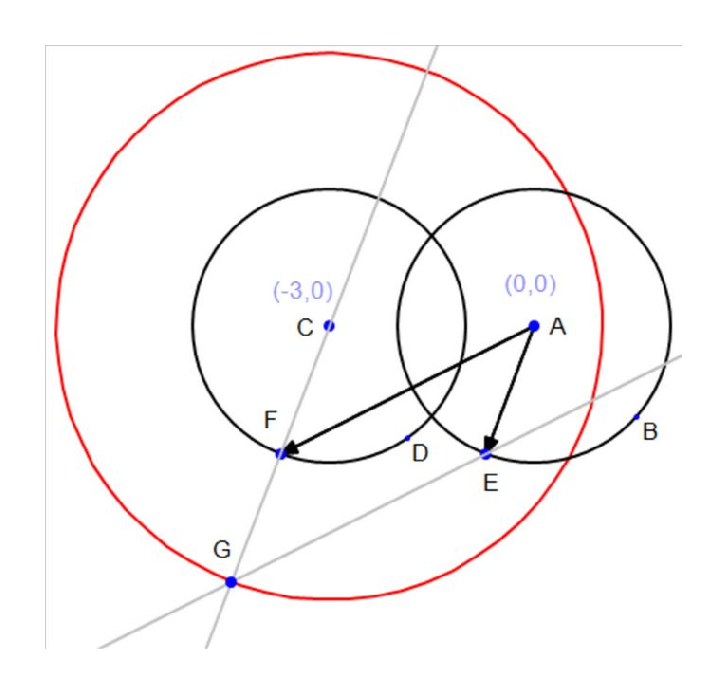
\includegraphics[width=1.7in,keepaspectratio]{PJH75H18.pdf}
\end{center}
 \caption{Circle and two fixed points.}
 \label{fig5}
\end{figure}

We consider two circles $C_{1}$ and $C_{2},$ whose centers are at $A$ and $C,
$ and the radii are $r_{1}$ and $r_{2}$ respectively. We let $E$ and $F$ be
two moving points on $C_{1}$ and $C_{2}$ respectively. If $G$ is the point
so that $AEGF$ forms a parallelogram, what is the locus of $G$?

It is easy to see that the points $G$ satisfy $\overrightarrow{OG}=\overrightarrow{OA}
+\overrightarrow{AG}=\overrightarrow{OA}+\left(  \overrightarrow
{AE}+\overrightarrow{AF}\right)  $ (see Figure~\ref{fig5}).
We observe that it is easier to solve this problem using vectors than
algebraically.

To simplify our problem a bit, assume $A=(0,0)$. The first
glance of the locus contains a surprise. The new locus (in red of both
parts of Figure~\ref{fig5})
is centered at the center $C$ of the second circle $C_2$ but with a
radius larger than $r_2$. The locus $\overrightarrow{OG}=\overrightarrow
{AE}+\overrightarrow{AF}$ can be written as $\overrightarrow{AE}+\left(
\overrightarrow{AC}+\overrightarrow{CF}\right)  =\left(  \overrightarrow
{AE}+\overrightarrow{AC}\right)  +\overrightarrow{CF}$. Note that $\left(
\overrightarrow{AE}+\overrightarrow{AC}\right)$ is a translation from the
circle $C_{1}$ to another circle centered at $C$ with the same radius $r_{1}$.
But the locus for $\left(  \overrightarrow{AE}+\overrightarrow{AC}\right)
+\overrightarrow{CF}$ becomes the circle centered at $C$ and radius is
$r_{1}+r_{2}$. This is clear if we take $C_{1}$ to be $[a+r\cos t, b+r\sin t]$ and
$C_{2}$ to be $[c+r_{2}\cos t, d+r_{2}\sin t]$. If $E$ and $F$ are two moving
points on $C_{1}$ and $C_{2}$ respectively, then it is clear that the locus
$\overrightarrow{OG}=\overrightarrow{OA}+$ $\overrightarrow{AE}+\overrightarrow{AF}
=\left[
\begin{array}
[c]{c}%
a\\
b
\end{array}
\right]  +\left[
\begin{array}
[c]{c}%
\left(  a+r\cos t\right)  -a\\
\left(  b+r\sin t\right)  -b
\end{array}
\right]  +\left[
\begin{array}
[c]{c}%
\left(  c+r_{2}\cos t\right)  -a\\
\left(  d+r_{2}\sin t\right)  -b
\end{array}
\right]  =\left[
\begin{array}
[c]{c}%
\left(  c+\left(  r+r_{2}\right)  \cos t\right) \\
\left(  d+\left(  r+r_{2}\right)  \sin t\right)
\end{array}
\right]$. It is clear that the locus in this case is a circle centered at
$(c,d)$ with radius $r+r_{2}.$ We see an animation from supplemental resource [S1]
that the locus in green is indeed a translation from $A$ to $C$ with radius
being the sum of the original two circles, we show a sequence of screen shots
below when $A=(-1,2),C=(2,3),r_{2}=1$ and $r$ is going from $0$ to $1$ as
following Figure~\ref{fig6}.
Additional exploration is provided in supplemental resource [S2].

\begin{figure}[htpb]
\begin{center}
\parbox[b]{1.9in}{\begin{center}
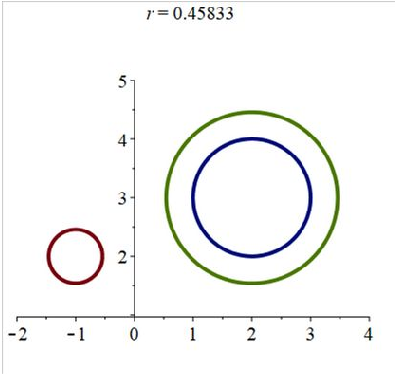
\includegraphics[height=1.7in,trim=0mm 0mm 0mm 12mm,clip,keepaspectratio]{PJH75H19-crop.pdf}
 \\ (a)
\end{center}}
\qquad
\parbox[b]{1.9in}{\begin{center}
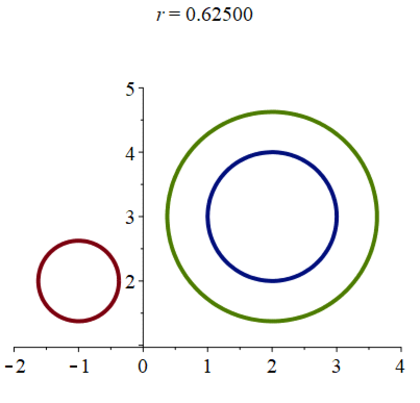
\includegraphics[height=1.7in,trim=0mm 0mm 0mm 10mm,clip,keepaspectratio]{PJH75H1A.pdf}
 \\ (b)
\end{center}}
\qquad
\parbox[b]{1.9in}{\begin{center}
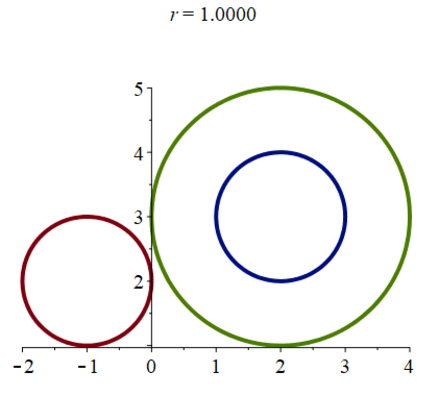
\includegraphics[height=1.7in,trim=0mm 0mm 0mm 10mm,clip,keepaspectratio]{PJH75H1B.pdf}
 \\ (c)
\end{center}}
\end{center}
\caption{Snapshots of the translation from $A=(-1,2)$ to $C=(2,3)$ when (a) $r=0.45833$, (b) $r=0.625$, and (c) $r=1$.}
\label{fig6}
\end{figure}

\textbf{Remark:}
We encourage readers to explore the generalization of the previous
example when the points $G$ satisfy
$\overrightarrow{OG}=\overrightarrow{OA}+$ $r\overrightarrow{AE}+s\overrightarrow{AF}$,
where $r$ and $s\in(0,1)$.

We now consider the scenario when the circles $C_1$ and $C_2$ are replaced by ellipses:

\begin{exercise} \label{ex5}
Given two fixed ellipses: $\frac{x^{2}}{4}+y^{2}=1$ (in blue) and
$\frac{\left(  x+1\right)  ^{2}}{2}+(y-1)^{2}=1$ (in black), centered at $O$
and $P$ respectively (see Figure~\ref{fig7} below). Let $A$ and $B$ be two moving points
on these two ellipses respectively. Find the locus for
$\overrightarrow{OA}+\overrightarrow{OB}$.
\end{exercise}

We leave it to the reader to verify that the locus is an ellipse centered at
$P$. In fact, the major and minor axes of the locus will be the sums
from the the respective lengths of the original two ellipses. In other
words, the equation of the locus should be
$\dfrac{\left(  x+1\right)^{2}}{\left(  2+\sqrt{2}\right)^{2}}+\dfrac{(y-1)^{2}}{(1+1)^2}=1$.

\begin{figure}[htbp]
\begin{center}
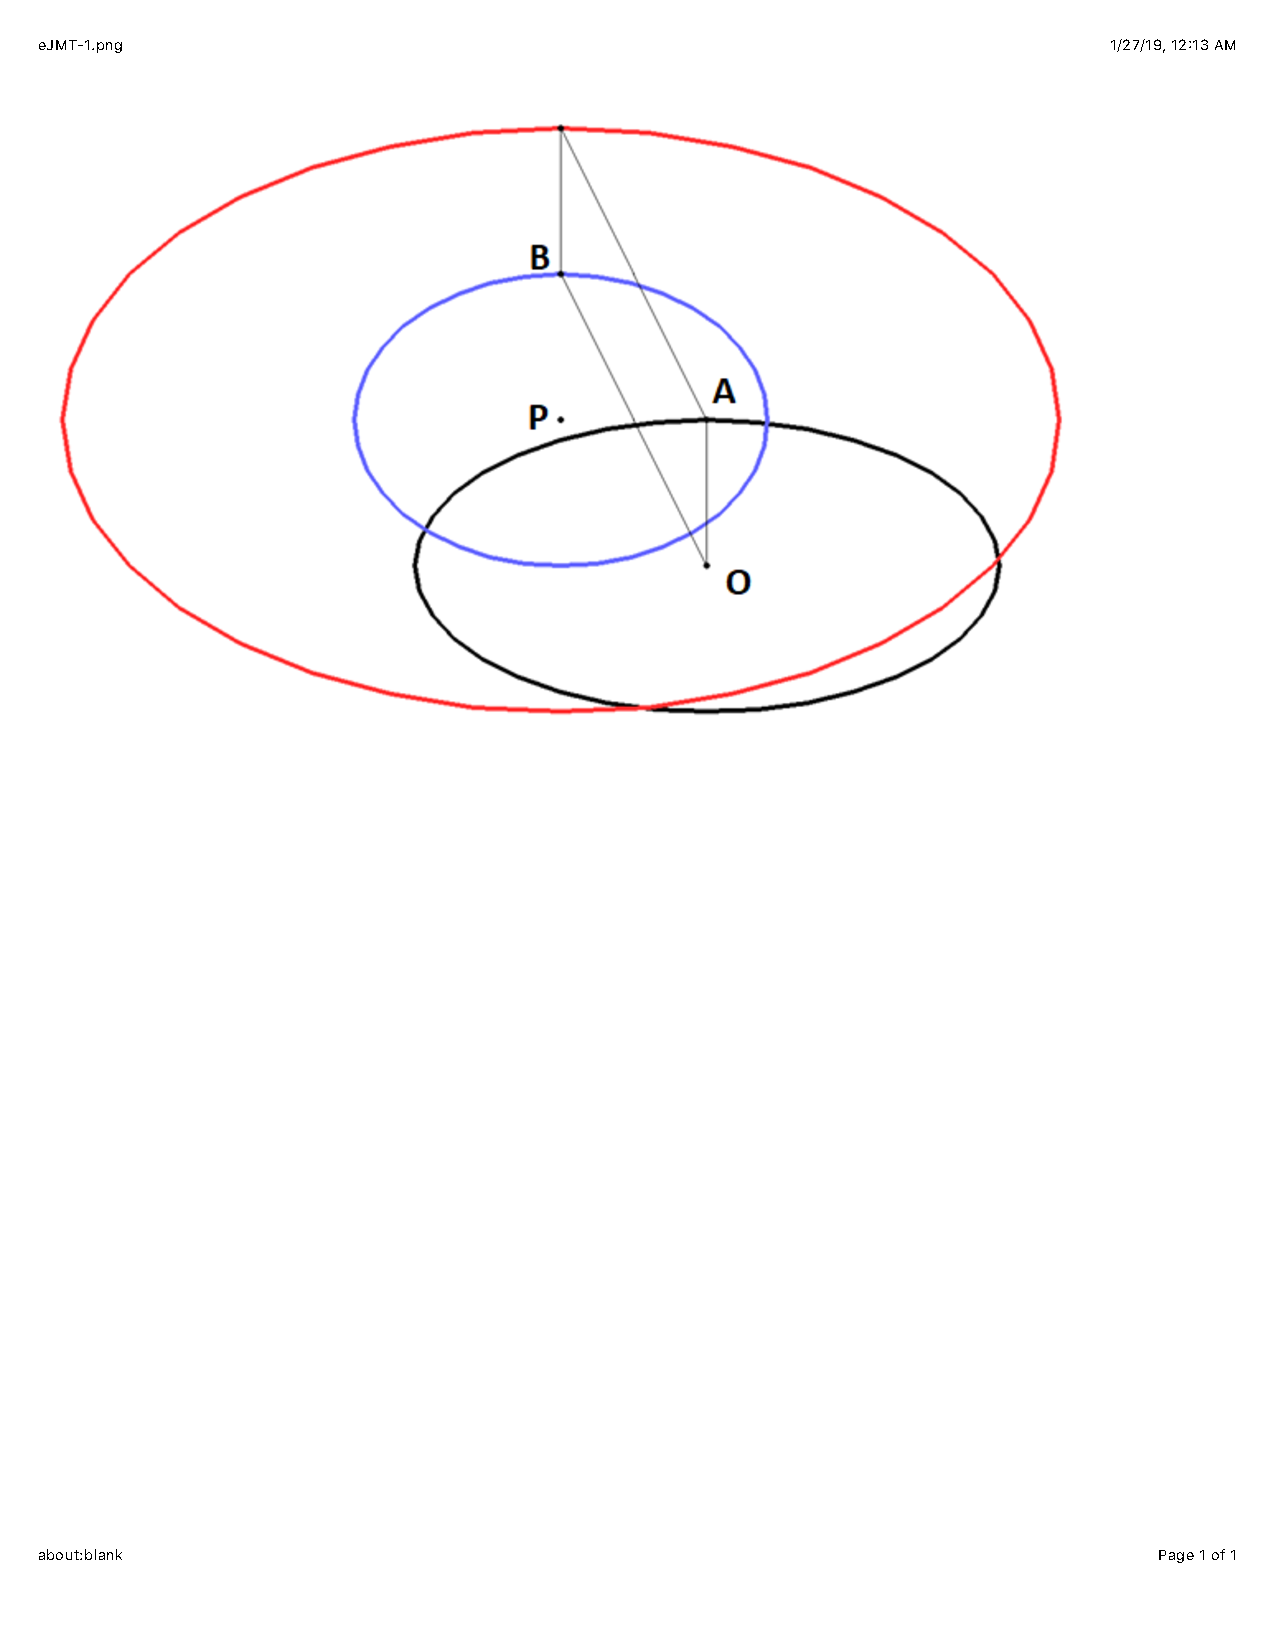
\includegraphics[height=1.7in,trim=0mm 120mm 35mm 15mm,clip,keepaspectratio]{eJMT-1.pdf}
\end{center}
 \caption{Locus and translation of an ellipse.}
 \label{fig7}
\end{figure}

\textbf{Remark:}
The locus in the preceding example can be viewed as a result of a
linear combinations from the original two ellipses.
Readers are encouraged to explore the problem of finding the locus of
$r\overrightarrow{OA}+s\overrightarrow{OB}$, where $r$ and $s\in(0,1)$.

\begin{exercise} \label{ex6}
We are given two fixed cardioid $[x_{1}(a,r,t),y_{1}(b,r,t)]=[a+(r-\cos t)\cos
t,b+(r-\cos t)\sin t]$ and $[x_{2}(c,r,t),y_{2}(d,r,t)]=[c+(r-\cos t)\cos
t,d+(r-\cos t)\sin t]$. Let $A$ and $B$ be two moving points on these two
cardioids respectively. Find the locus for $\overrightarrow{OA}%
+\overrightarrow{OB}$.
(A solution to this problem can be found in supplemental resources [S2], [S6] or [S9].)
\end{exercise}

\subsection{Locus of three moving points} \label{sec3-2}

We now explore finding a locus when there are three moving points on three
separate closed curves. It is surprisingly simple to find the locus using
vectors in this case once we know the given (parametric) equations of the
three closed curves.

First, recall that the implicit form for the ellipse centered
at $(c_x, c_y)$ with major axis $r_x$ and minor axis $r_y$ and rotated by
the angle $\alpha$ is

\[
\frac{\left(  \left(  x-c_{x}\right)  \cos\alpha+\left(  y-c_{y}\right)
\sin\alpha\right)  ^{2}}{r_{x}^{2}}+\frac{\left(  \left(  x-c_{x}\right)
\sin\alpha-\left(  y-c_{y}\right)  \cos\alpha\right)  ^{2}}{r_{y}^{2}}=1.
\]
The corresponding parametric representation of this rotated ellipse is,
for each $0\le \theta\le 2\pi$,
\begin{align*}
x(\theta)  & =c_{x}+r_{x}\cos\alpha\cos\theta-r_{y}\sin\alpha\sin\theta,\\
y(\theta)  & =c_{y}+r_{x}\sin\alpha\cos\theta+r_{y}\cos\alpha\sin\theta.
\end{align*}
So, for example

\begin{example} \label{ex7}
Let $C_1$ be the ellipse $\frac{\left(x+2\right)^{2}}{4}+(y-1)^{2}=1$
rotated by the angle of $\alpha=120$ degrees. The center of this
ellipse is
$(-2,1)$, the major radius is $2$ and minor radius is $1$. We write the
parametric equation $C_{1}$ as follows:
\begin{align*}
x_{1}(\theta)  & =-2+2\cos\left(  \frac{2\pi}{3}\right)  \cos\theta
-\sin\left(  \frac{2\pi}{3}\right)  \sin\theta,\\
y_{1}(\theta)  & =1+2\sin\left(  \frac{2\pi}{3}\right)  \sin\theta+\cos\left(
\frac{2\pi}{3}\right)  \sin\theta,
\end{align*}
where $\theta\in\left[  0,2\pi\right]$. Let the second curve be the cardioid
$C_{2}$: $r=1-\cos\theta$, for $\theta\in\left[  0,2\pi\right]$. Thus,
a parametric representation of $C_{2}$ is
\begin{align*}
x_{2}\left(  \theta\right)   & =\left(  1-\cos\theta\right)  \cos\theta,\\
y_{2}\left(  \theta\right)   & =\left(  1-\cos\theta\right)  \sin\theta,
\end{align*}
where $\theta\in\left[  0,2\pi\right]$. And, let the third curve $C_3$
be the unit circle centered at the point $(2,2)$:
\begin{align*}
x_{3}(\theta)  & =2+\cos\theta,\\
y_{3}(\theta)  & =2+\sin\theta,
\end{align*}
where $\theta\in\left[  0,2\pi\right]$. Let $I$, $F$, and $G$ be three moving
points on $C_{1},C_{2}$ and $C_{3}$, respectively. The goal is to find the
locus of $\overrightarrow{IF}+\overrightarrow{IG}$.
\end{example}

If the locus points are called $J$, then the problem is to describe the 
vectors $\overrightarrow{OJ}=\overrightarrow{OI}+\overrightarrow{IJ}$,
where $\overrightarrow{IJ}=\overrightarrow{IF}+\overrightarrow{IG}$,
\[
\overrightarrow{IF}=\left[
\begin{array}
[c]{c}%
x\left(  \theta\right) \\
y\left(  \theta\right)
\end{array}
\right]  =\left[
\begin{array}
[c]{c}%
\left(  1-\cos\theta\right)  \cos\theta-\left[  -2+2\cos\left(  \frac{2\pi}%
{3}\right)  \cos\theta-\sin\left(  \frac{2\pi}{3}\right)  \sin\theta\right] \\
\left(  1-\cos\theta\right)  \sin\theta-\left[  1+2\sin\left(  \frac{2\pi}%
{3}\right)  \sin\theta+\cos\left(  \frac{2\pi}{3}\right)  \sin\theta\right]
\end{array}
\right],
\]
and
\[
\overrightarrow{IG}=\left[
\begin{array}
[c]{c}%
x\left(  \theta\right) \\
y\left(  \theta\right)
\end{array}
\right]  =\left[
\begin{array}
[c]{c}%
2+\cos\theta-\left[  -2+2\cos\left(  \frac{2\pi}{3}\right)  \cos\theta
-\sin\left(  \frac{2\pi}{3}\right)  \sin\theta\right] \\
2+\sin\theta-\left[  1+2\sin\left(  \frac{2\pi}{3}\right)  \sin\theta
+\cos\left(  \frac{2\pi}{3}\right)  \sin\theta\right]
\end{array}
\right]  .
\]
We use Maple \cite{Maple} to show the locus of the points $J$ in red,, emphasizing
the construction of the points corresponding to $t=0$ and to $t=\pi$ in
Figures~\ref{fig8}(a) and \ref{fig8}(b), respectively.
In particular, these snapshots clearly demonstrate that $\overrightarrow{IJ}$ is a result
of linear combination of $\overrightarrow{IF}$ and $\overrightarrow{IG}$.

With the use of a CAS, such as Maple \cite{Maple}, it is easy to generate
animations when the weights in the linear combination are allowed to be $r$ or $s$,
where each value is between $0$ and $1$.
For example, Figures~\ref{fig8}(c) and \ref{fig8}(d) demonstrate the locus when
$( r, s )  = ( 0.54167, 1 )$ and $( r, s )=( 0.5, 0.20833 )$, respectively.
Please see supplemental resource [S3] for more details and explorations.

\begin{figure}
\begin{center}
\parbox[b]{2.8in}{\begin{center}
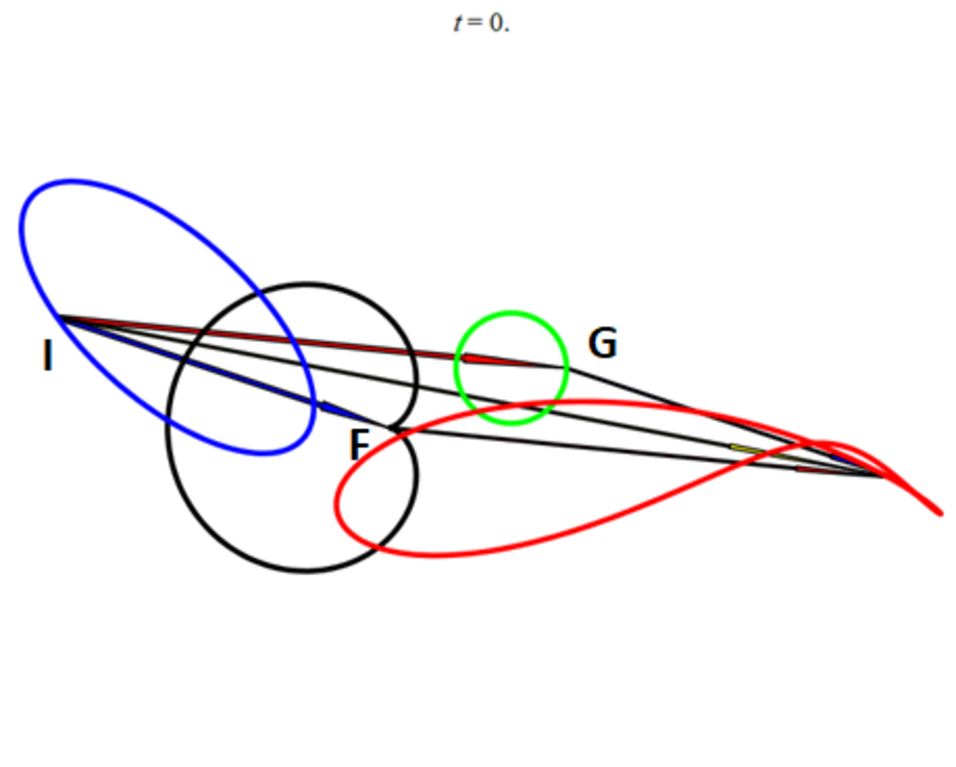
\includegraphics[height=2.0in,trim=0mm 0mm 0mm 15mm,clip,keepaspectratio]{IF+IG-crop.pdf}
\\
(a)
\end{center}}
\qquad
\parbox[b]{2.8in}{\begin{center}
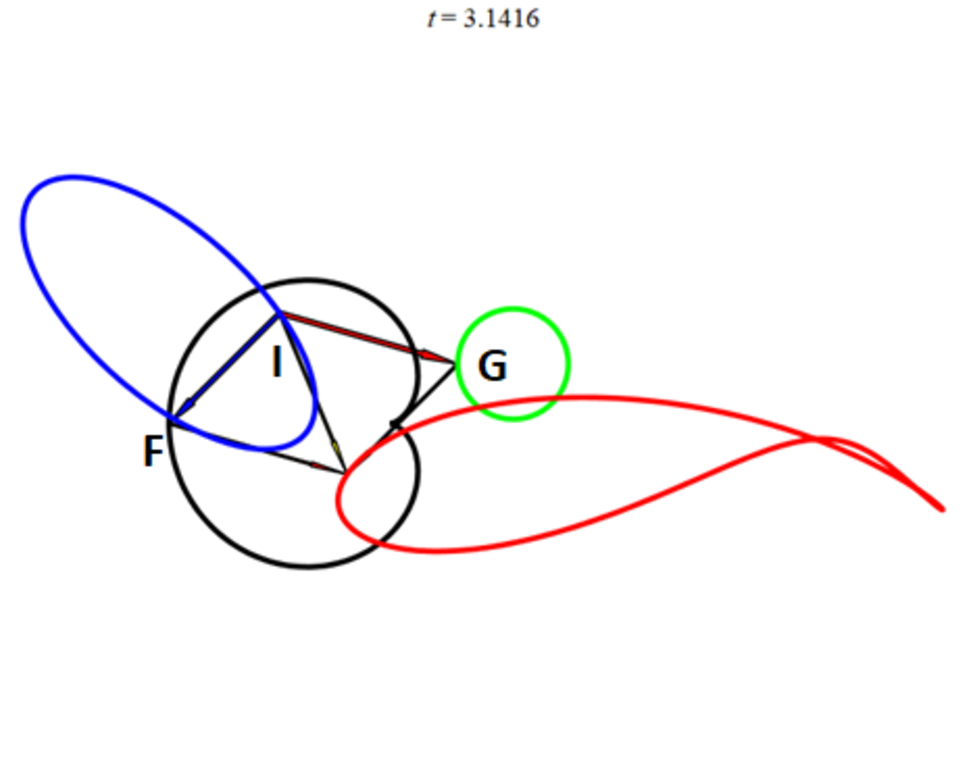
\includegraphics[height=2.0in,trim=0mm 0mm 0mm 15mm,clip,keepaspectratio]{IF+IG_Pi-crop.pdf}
\\
(b)
\end{center}}
\\
\parbox[b]{2.8in}{\begin{center}
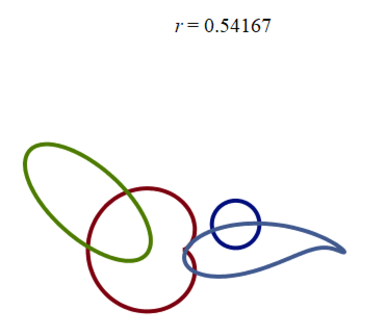
\includegraphics[height=2.0in,trim=0mm 0mm 0mm 15mm,clip,keepaspectratio]{PJH75H1C-crop.pdf}
\\
(c)
\end{center}}
\qquad
\parbox[b]{2.8in}{\begin{center}
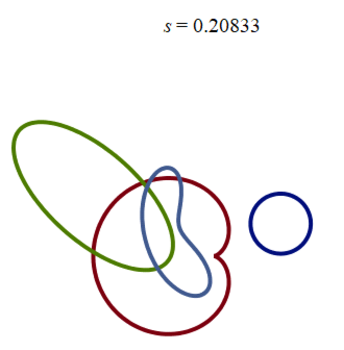
\includegraphics[height=2.0in,trim=0mm 0mm 0mm 15mm,clip,keepaspectratio]{PJH75H1D-crop.pdf}
\\
(d)
\end{center}}
\end{center}
\caption{Snapshots showing the construction of the point $J$ at (a) $t=0$ and (b) $t=pi$.
               Also, the entire locus of  the point $J$
               when (c) $r=0.54167$ and $s=1$ and (d) $r=\frac{1}{2}$ and $s=0.20833$.
}
\label{fig8}
\end{figure}

\textbf{Discussion: }
In the preceding example, the locus is a closed curve $C_{4}$
that can be determined once we are given the three closed curves,
$C_{1}$, $C_{2}$, and $C_{3},$ and properly setting up the linear combinations of vectors. One
application of this will be using the light source at a point on either
$C_{1}$, $C_{2}$, or $C_{3}$, and we need to find the caustic curve of $C_{4},$
which we call it $C_{5}.$ We can continue this process by finding a sequence of
closed curves, $C_{4}$, $C_{5}$, ... so that $C_{n+1}$ depends on $C_{n}$, where
$n\geq3$, which we can imagine finding each $C_{n}$ becomes more computational
intensive when $n$ increases.

Now we consider the locus resulting from four closed surfaces in 3D, three of which
are originated from the preceding 2D example. Suppose surface $S_{1}$ has a
parametric representation as
\begin{align*}
x_{1}(t_{1},t_{2})
  & =\left(  x_{1}\left(  t_{1}\right)  +2\right)  \sin t_{2}-2\\
  & =-2+\left(  2\cos\left(  \frac{2\pi}{3}\right)  \cos t_{1}
        -\sin\left(\frac{2\pi}{3}\right)  \sin t_{1}\right)  \sin t_{2},\\
y_{1}\left(  t_{1},t_{2}\right)
  & =\left(  y_{1}\left(  t_{1}\right)-1\right)  \sin t_{2}+1\\
  & =1+\left(  2\sin\left(  \frac{2\pi}{3}\right)  \sin\theta+\cos\left(\frac{2\pi}{3}\right)  \sin\theta\right)  \sin t_{2},\\
z_{1}(t_{1},t_{2})
  & =\cos\left(  t_{2}\right)  ,
\end{align*}
where $t_{1}\in\left[  0,2\pi\right]  $ and $t_{2}\in\left[  0,\pi\right]$.
The surface $S_{2}$ is given by rotating the curve
$\left[  x_{2}\left(t_{1}\right)  ,y_{2}(t_{1})\right]  $ around the $x-axis$ as follows:
\begin{align*}
x_{2}\left(  t_{1},t_{2}\right)
  & =x_{2}\left(  t_{1}\right) \\
y_{2}\left(  t_{1},t_{2}\right)
  & =y\left(  t_{1}\right)  \cos t_{2}\\
  & =\left(  1-\cos t_{1}\right)  \sin t_{1}\cos t_{2}\\
z_{2}(t_{1},t_{2})
  & =y\left(  t_{1}\right)  \sin t_{2}\\
  & =\left(  1-\cos t_{1}\right)  \sin t_{1}\sin t_{2},
\end{align*}
where $t_{1},t_{2}\in\left[  0,2\pi\right]$. And, the surfaces $S_{3}$ and $S_4$
are taken to be spheres with radius $1$ and centers $(1,1,1)$ and $(1,-1,-1)$,
respectively. As such, $S_{3}$ and $S_{4}$ are written parametrically as:
\begin{align*}
&x_{3}(t_{1},t_{2})
  =1+\sin t_{2}\cos t_{1},
&&y_{3}(t_{1},t_{2})
  =1+\sin t_{2}\sin t_{1},
&&z_{3}(t_{1},t_{2})
  =1+\cos t_{2},\\
&x_{4}(t_{1},t_{2})
 =1+\sin t_{2}\cos t_{1},
&&y_{4}(t_{1},t_{2})
  =-1+\sin t_{2}\sin t_{1},
&&z_{4}(t_{1},t_{2})
 =-1+\cos t_{2},
\end{align*}
where $t_{1},t_{2}\in\left[  0,2\pi\right]$.
If we let $A$, $B$, $C$, $D$ denote the four
moving points on $S_{1}$, $S_{2}$, $S_{3}$, and $S_{4}$, respectively,
then the locus of interest consists of the points $E$ such that
$\overrightarrow{OE}=\overrightarrow{OA}+( \overrightarrow{AB}
                                 +\overrightarrow{AC}+\overrightarrow{AD})$.
In this form the locus is easily calculated and plotted (see Figure~\ref{fig9}(d)).

We see $S_{1}$ is a rotated ellipsoid shown in yellow (see Figure~\ref{fig9}(a)),
$S_{2}$ is a surface shown in blue which rotates
the cardioid $[x_{2}(t_{1}), y_{2}(t_{1})]$ around the $x$-axis (see Figure~\ref{fig9}(b)).
Figure~\ref{fig9}(c) shows all four surfaces, including the spheres $S_{3}$
and $S_{4}$ in red and magenta, respectively.
We depict, in Figure~\ref{fig9}(d), the locus of the points $E$ satisfying
$\overrightarrow{OE}=\overrightarrow{OA}+\left(\overrightarrow{AB}+\overrightarrow{AC}+\overrightarrow{AD}\right)$
in green.
Please see supplemental resource [S3] for more details.
We encourage the readers to explore the locus of linear combinations of vector
$\overrightarrow{OE}=\overrightarrow{OA}+r\overrightarrow{AB}
                                +s\overrightarrow{AC}+t\overrightarrow{AD}$,
where $r$, $s$, and $t\in\left(  0,1\right)$.

\begin{figure}
\begin{center}
\parbox[b]{1.6in}{\begin{center}
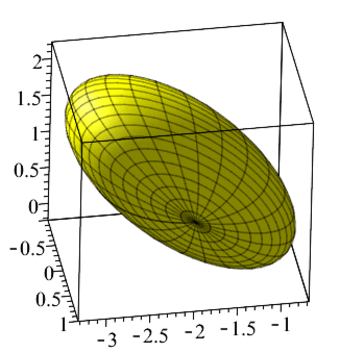
\includegraphics[height=1.7in]{PJH75H1E.pdf}
\\
(a)
\end{center}}
\qquad
\parbox[b]{1.6in}{\begin{center}
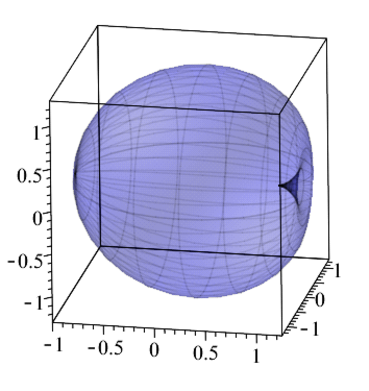
\includegraphics[height=1.7in]{PJH75H1F.pdf}
\\
(b)
\end{center}}
\\
\parbox[b]{1.6in}{\begin{center}
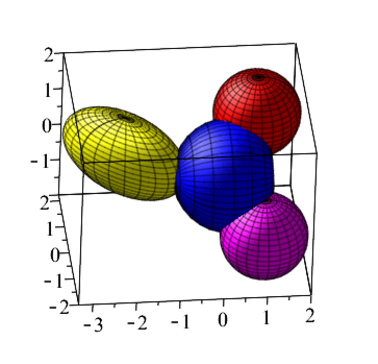
\includegraphics[height=1.7in]{PJH75H1G.pdf}
\\
(c)
\end{center}}
\qquad
\parbox[b]{1.6in}{\begin{center}
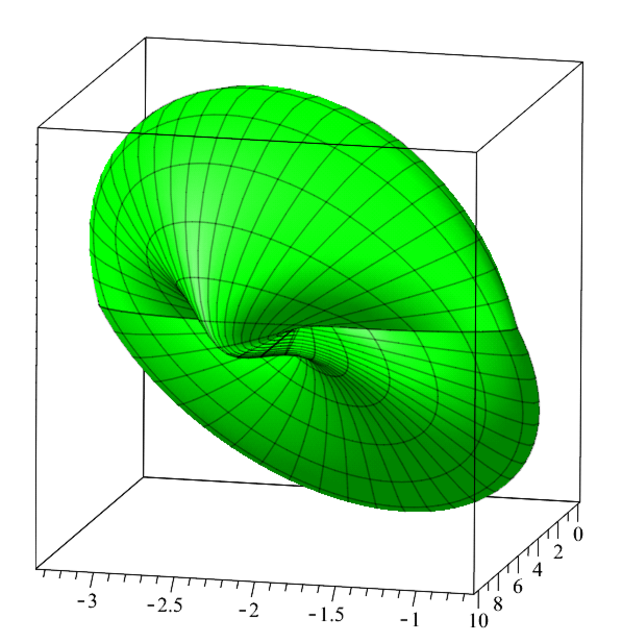
\includegraphics[height=1.7in]{PJH75H1H.pdf}
\\
(d)
\end{center}}
\end{center}
\caption{(a) The surface $S_1$.
              (b) The surface $S_2$.
              (c) The surfaces $S_1$ (yellow), $S_2$ (blue), $S_3$ (red), and $S_4$ (magenta).
              (d) Locus of linear combinations of surfaces $S_1$, $S_2$, $S_3$, and $S_4$.}
\label{fig9}
\end{figure}

\section{Locus When Fixing Two Points On A Curve} \label{sec4}

In this section we discuss a locus problem that is inspired by the following
college entrance exam practice problem from China (see \cite{Gao}).

\begin{example} \label{ex8}
Given a fixed ellipse, say $\frac{x^{2}}{a^{2}}+\frac{y^{2}}{b^{2}}=1$
($a>0$ and $b>0$),
where $BE$ is the major axis and $F$ is a moving point on the ellipse,
construct two lines passing through $B$ and $E$, respectively, that
intersect at the point $I$ such that
$\measuredangle IBF=\measuredangle FEI=90^{\circ}$ (see Figure~\ref{fig10}).
Let $J$ be the midpoint of $BI$, find the locus of $J$.
[Note that the red curve represents the scattered plot of $J$
that can be traced by using ClassPad \cite{CP}.]%

\begin{figure}[htpb]
\begin{center}
\parbox[b]{2.4in}{\begin{center}
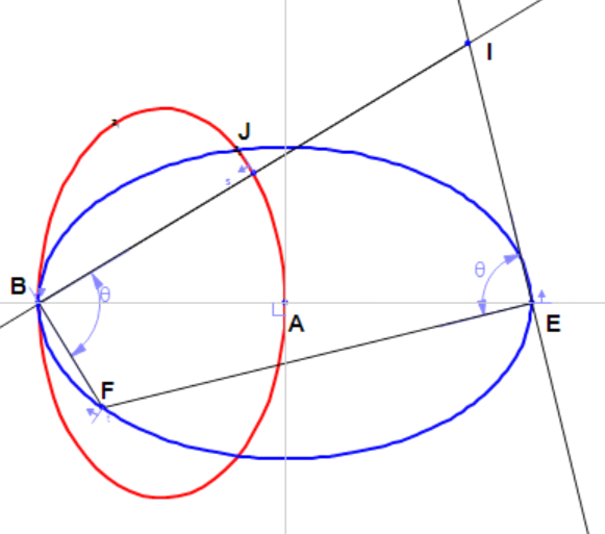
\includegraphics[height=2.1in,keepaspectratio]{PJH75H1I.pdf}
 \\ (a)
\end{center}}
\qquad
\parbox[b]{2.4in}{\begin{center}
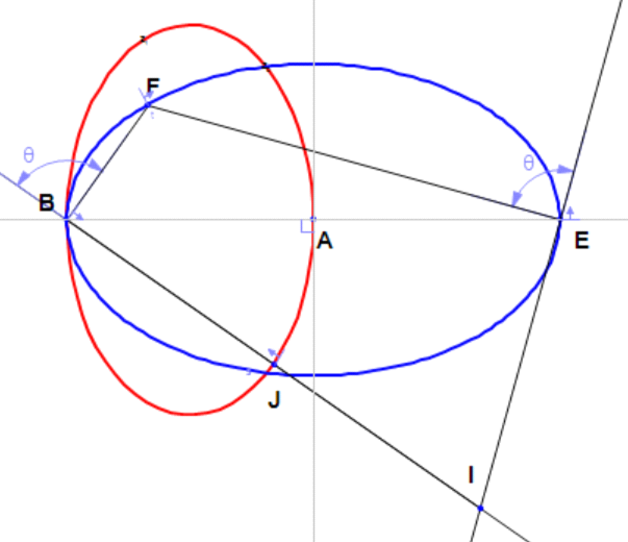
\includegraphics[height=2.1in,keepaspectratio]{PJH75H1J.pdf}
 \\ (b)
\end{center}}
\end{center}
\caption{Ellipse, two fixed points, and the points $J$
         when (a) $t=t_1$ and (b) $t=t_2$.}
\label{fig10}
\end{figure}
\end{example}

We remark here that if, instead of appearing as a question on an entrance
exam, this problem is presented in the context of a mathematics experiment
class with access to technological tools to enhance visualization, more
students would have enjoyed the experience, and they would actually learn
some useful mathematics. For example, before deriving an analytic answer
to this question they can play and learn what a locus might look like.
In this way the learning process becomes much more enjoyable.
Here are some explicit steps showing ways to explore this problem.

\begin{enumerate}
\item Start with a DGS (say \cite{CP} in this case) for necessary geometric
constructions and next use the scattered plot to conjecture what the locus
should look like. Further experiment with a symbolic DGS such as \cite{GE}
to generate a possible symbolic solution.

\item Solve the problem analytically by hand for simple scenario or solve it
analytically with a CAS such as \cite{Maple} as the problem becomes more
algebraically intensive.
\end{enumerate}

We first present how one may solve this simple case by hand --- without the
use of technology. We let $B=(-a,0)$, $E=(a,0)$, and the moving
point on the ellipse $F=(x_{0},y_{0})$. We denote the slopes of $FB$ and $FE$
to be $k_{FB}$ and $k_{FE}$, respectively; then
$k_{FB}=\frac{y_{0}}{x_{0}+a}$ and $k_{FE}=\frac{y_{0}}{x_{0}-a}$.
Thus, the equations for lines $BI$ and $EI$ are%
\begin{equation}
y=-\frac{x_{0}+a}{y_{0}}\left(  x+a\right) \label{eq1}%
\end{equation}
and
\begin{equation}
y=-\frac{x_{0}-a}{y_{0}}\left(  x-a\right), \label{eq2}%
\end{equation}
respectively. Substituting (\ref{eq1}) into (\ref{eq2}) yields:
\begin{align*}
-\frac{x_{0}+a}{y_{0}}\left(  x+a\right)   & =-\frac{x_{0}-a}{y_{0}}\left(
x-a\right) \\
\left(  x_{0}+a\right)  \left(  x+a\right)   & =\left(  x_{0}-a\right)
\left(  x-a\right) \\
2ax+2ax_{0}  & =0.
\end{align*}
Since $a>0$, this requires $x=-x_0$ and so the point of intersection is
$I=(-x_{0},\allowbreak-\frac{1}{y_{0}}\left(  a+x_{0}\right)  \left(
a-x_{0}\right)$.
The midpoint for $BI$ is thus
\[
J=\left(  X,Y\right)  =\left(  \frac{-x_{0}-a}{2},-\frac{1}{2y_{0}}\left(
a+x_{0}\right)  \left(  a-x_{0}\right)  \right)  .
\]
This implies that $Y=\frac{a-x_0}{y_{0}}X$. To obtain the parametric form
for the locus $J$, note that since $(x_0, y_0)$ is a point on the ellipse,
$\frac{x_{0}^{2}}{a^{2}}+\frac{y_{0}^{2}}{b^{2}}=1$, and so
$x_{0}=a\cos t$ and $y_{0}=b\sin t$ for some $t\in[0,2\pi)$.
The parametric equations for the locus of $J$ is found to be
\[
\left\{
\begin{array}
[c]{c}%
X(t) =\dfrac{-a\cos t-a}{2}=\dfrac{-a(\cos t+1)}{2}\\
Y(t) =\dfrac{(a-a\cos t)}{b\sin t}=\dfrac{a(1-\cos t)}{b\sin t} X
\end{array}
\right.  .
\]

\textbf{Exploration 1:}
It is not difficult to generalize this problem to ask for
the locus $J=(X,Y)$ satisfying $\overrightarrow{BJ}=s\overrightarrow{BI}$ for
some real number $s\in[0,1]$.
In view of $\overrightarrow{BJ}=s\overrightarrow{BI}$, we have
\begin{align*}
(X+a,Y)  & =s\left(  -x_{0}+a,-\frac{1}{y_{0}}\left(  a+x_{0}\right)  \left(
a-x_{0}\right)  \right) \\
J  & =\left(  X,Y\right)  =\left(  -s(x_{0}-a)-a\right)  ,\allowbreak\frac
{s}{y_{0}}\left(  x_{0}+a\right)  \left(  x_{0}-a\right).
\end{align*}

As before, $\frac{x_{0}^{2}}{a^{2}}+\frac{y_{0}^{2}}{b^{2}}=1$
and we set $x_{0}=a\cos t$ and $y_{0}=b\sin t$, where $t\in[0,2\pi)$,
to obtain the parametric equations for the locus $J$ to be
\begin{align}
X  & =-s( a\cos t-a) -a                                   \label{Locus J}\\
Y  & =\frac{s\left((a\cos t)^{2}-a^{2}\right)  }{b\sin t}.\nonumber
\end{align}

\textbf{Remarks: }
\begin{enumerate}
\item We can use the DGS Geometry Expressions \cite{GE} to construct
      the locus $J$ above through geometry constructions.
      We depict some screen shots when $s=0.25$ and $0.75$ in the
      following Figures 11(a) and 11(b).

\item
The analytic derivation leading to \ref{Locus J} should be equivalent to
the geometric construction obtained using Geometry Expressions \cite{GE}.
The to representations are graphed in Figure~\ref{fig11}. The similarities
in these figures suggest that these representations are equivalent.
The CAS Maple \cite{Maple} is useful in verifying that the two representations
are, in fact, equivalent.

\begin{figure}[htpb]
\begin{center}
\parbox[b]{2.2in}{\begin{center}
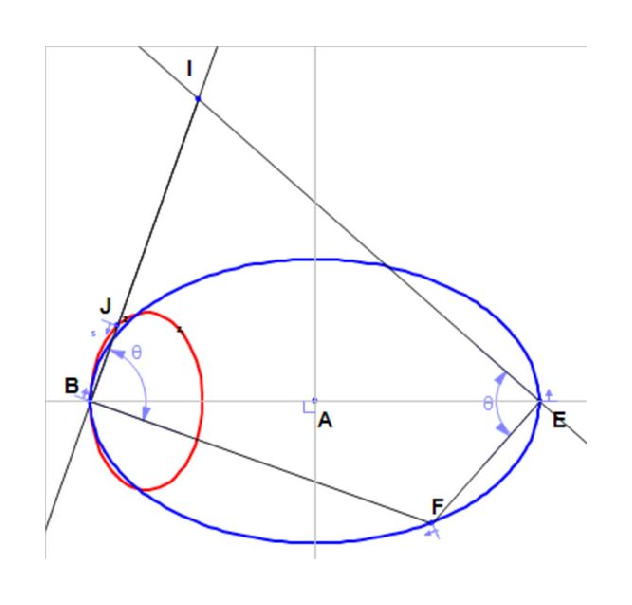
\includegraphics[height=2.1in,keepaspectratio]{PJH75I1K.pdf}
 \\ (a)
\end{center}}
\qquad
\parbox[b]{2.2in}{\begin{center}
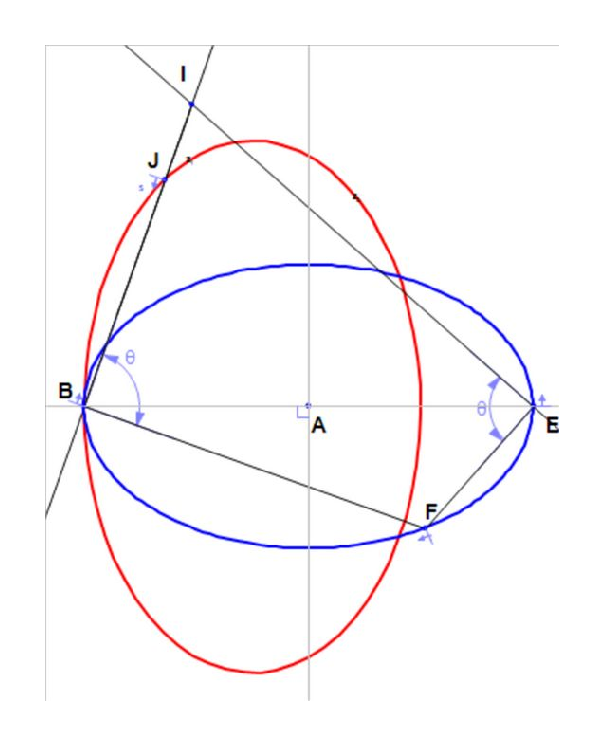
\includegraphics[height=2.1in,keepaspectratio]{PJH75I1L.pdf}
 \\ (b)
\end{center}}
\end{center}
\caption{Locus of the points $J$ for (a) $s=\frac{1}{4}$ and (b) $s=\frac{3}{4}$.}
\label{fig11}
\end{figure}

\end{enumerate}

\textbf{Exploration 2:}
Consider the scenario in which instead of requiring the
$\measuredangle IBF=\measuredangle FEI=\theta$ for some given angle $\theta$
(not necessarily a right angle).
Let $B=(-a,0)$, $E=(a,0)$, and denote the moving point on the ellipse
by $F=(x_{0},y_{0})$. Denoting the slopes of $FB$ and $FE$
as $k_{FB}$ and $k_{FE}$, respectively, then
$k_{FB}=\frac{y_{0}}{x_{0}+a}=\tan\theta_{1}$
and
$\theta_{1}=\tan^{-1}\left(  \frac{y_{0}}{x_{0}+a}\right)$.
In the meantime, $k_{FE}=\frac{y_{0}}{x_{0}-a}=\tan\theta_{2}$
and $\theta_{2}=\tan^{-1}\left(  \frac{y_{0}}{x_{0}-a}\right)$.

The equations for lines $BI$ and $EI$ are found,
with the help of Maple \cite{Maple}, to be:
\begin{equation}
y=\tan\left(  \tan^{-1}\left(  \frac{y_{0}}{x_{0}+a}\right)  +\theta\right)
\left(  x+a\right) \label{eq5}
\end{equation}
and
\begin{equation}
y=\tan\left(  \tan^{-1}\left(  \frac{y_{0}}{x_{0}-a}\right)  -\theta\right)
\left(  x-a\right) \label{eq6}%
\end{equation}
respectively.
Using (\ref{eq5}) and (\ref{eq6}) to solve for $x$ yields
\[
x=\frac{a\tan\left(  \arctan\left(  \frac{y_{0}}{-x_{0}+a}\right)
+\theta\right)  -\tan\left(  \arctan\left(  \frac{y_{0}}{x_{0}+a}\right)
+\theta\right)  }{\tan\left(  \arctan\left(  \frac{y_{0}}{x_{0}+a}\right)
+\theta\right)  +\tan\left(  \arctan\left(  \frac{y_{0}}{-x_{0}+a}\right)
+\theta\right)  },
\]
and use (\ref{eq5}) or (\ref{eq6}) to find an expression for $y$,
which is too long to display and can be found in supplemental resource [S4].
To obtain parametric equations for the locus of $J=(X_1,Y_1)$ such that
$\overrightarrow{BJ} = s \overrightarrow{BI}$, $s\in[0,1]$,
where $I=(x,y)$ is the intersection of $BI$ and $EI$, substitute
$x_{0}=a\cos t$ and
$y_{0}=b\sin t$ for $x$ and $y$, respectively.
Then we see that the locus of $J$ can be expressed as

\begin{align*}
\left[
\begin{array}
[c]{c}%
X_{1}\left(  a,b,s,t,\theta\right) \\
Y_{1}\left(  a,b,s,t,\theta\right)
\end{array}
\right]
 & = \left[
\begin{array}
[c]{c}%
s\left(  x\left(  a,b,s,t,\theta\right)  +a\right)  -a\\
sy\left(  a,b,s,t,\theta\right)
\end{array}
\right] \\ 
 & = s\left[
\begin{array}
[c]{c}%
x\left(  a,b,s,t,\theta\right) \\
y\left(  a,b,s,t,\theta\right)
\end{array}
\right]  -\left(  1-s\right)  \left[
\begin{array}
[c]{c}%
a\\
0
\end{array}
\right]  .
\end{align*}

The actual expressions for $X_1(a,b,s,t,\theta)$ and $Y_1(a,b,s,t,\theta)$
 produced by Maple \cite{Maple} are shown in the following screenshots:

\begin{align*}
&
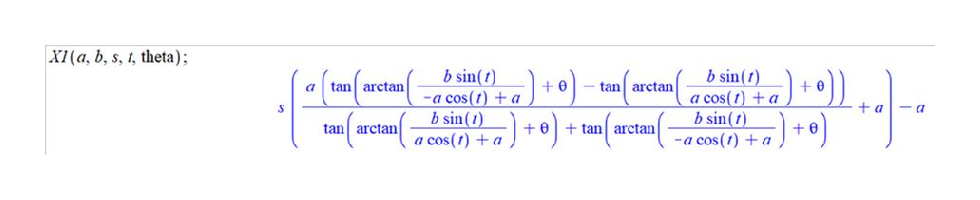
\includegraphics[width=\textwidth,keepaspectratio]{PJH75I1M.pdf}
\\
&
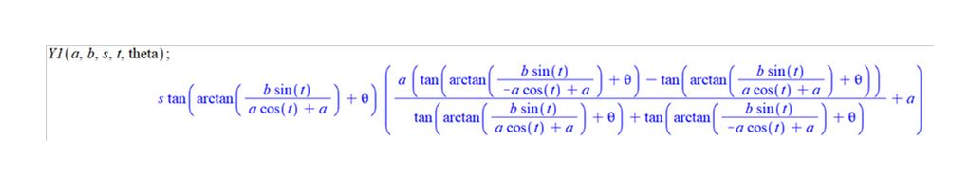
\includegraphics[width=\textwidth,keepaspectratio] {PJH75I1N.pdf}
\end{align*}

For comparison, Geometry Expressions \cite{GE} reports the corresponding
parametric equations for the locus of the point $J$ as, after simplification,
\begin{align*}
X &= s \frac{2a^2 b \cos(t)}{(a^2-b^2)\sin(2\theta)\sin(t)+2ab\cos(2\theta)} - (1-s)a
\\
Y &= s \frac{2a\left(a^2 \sin^2(\theta)+b^2\cos^2(\theta)\right) \sin(t) + ab\sin(2\theta)}{(a^2-b^2)\sin(2\theta)\sin(t)+2ab\cos(2\theta)}
\end{align*}

\textbf{Remark:}
The DGS Geometry Expressions \cite{GE} has the capability of
linking its outputs to a CAS such as \cite{Maple} for further computation.
Although it is not trivial to prove algebraically that the locus equation
$[X_{1},Y_{1}]$ obtained from Maple is identical to that of
$[X,Y]$ obtained from the Geometry Expressions, the Maple worksheet used
by the authors to check these results is provided as supplemental resources
[S4]; see all [S7] or [S10] for additional hands-on explorations.
These also provide graphical verifications under different scenarios:
varying one parameter, varying one parameter and fixing the other.
The two parts of Figure~\ref{fig12} show both $[X_1,Y_1]$ and $[X,Y]$
when $a=2$, $b=2$, $s=\frac{1}{4}$, and (a) $\theta=\frac{\pi}{4}$
and (b) $\theta=\frac{2\pi}{3}$.

\begin{figure}[htpb]
\begin{center}
\parbox[b]{2.5in}{\begin{center}
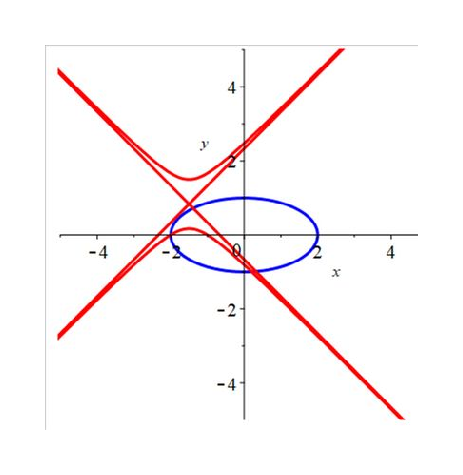
\includegraphics[height=2.5in,keepaspectratio]{PJH75I1O.pdf}
 \\ (a)
\end{center}}
\qquad
\parbox[b]{2.5in}{\begin{center}
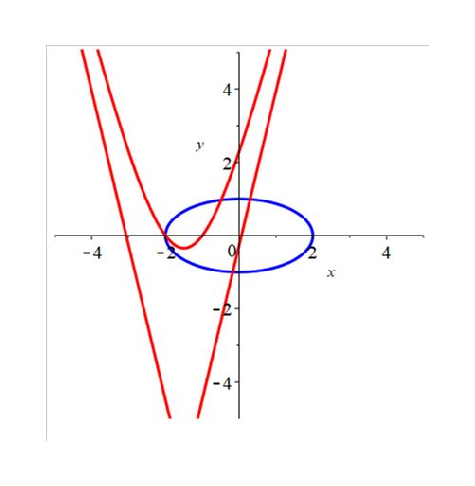
\includegraphics[height=2.5in,keepaspectratio]{PJH75I1P.pdf}
 \\ (b)
\end{center}}
\end{center}
\caption{Parametric curves $[X(2,2,\frac{1}{4},t,\theta), Y(2,2,\frac{1}{4},t,\theta)] 
                                          = [X_1(2,2,\frac{1}{4},t,\theta), Y_1(2,2,\frac{1}{4},t,\theta)]$
              for (a) $\theta=\frac{\pi}{4}$ and (b) $\theta=\frac{2\pi}{3}$}
\label{fig12}
\end{figure}

\subsection{Another Generalization: Replacing the Ellipse by a Cardioid} \label{ssec4-1}

Assuming technological tools are available to learners, it is natural to ask
what if the ellipse, discussed earlier, is replaced by another curve, say a
cardioid. In particular, we consider the following

\begin{example} \label{ex9}
We are given the cardioid $r=1-\cos t,t\in\lbrack0,2\pi]$ in Figure~\ref{fig13}.
Suppose the moving point $C$ is on the cardioid and two lines passing through
$B=(0,0)$ and $A=(a,0)$ respectively, and intersect at $G$ so that the angles
$\measuredangle CAG=\measuredangle CBG=90^{\circ}$.
Find the locus of the midpoint, $J$, of $AG$.
[Note, in Figure~\ref{fig13}, the red curve is a scattered plot
of the locus of $J$,
when $A=\left(  -2,0\right)$, and has been obtained using
\cite{CP}]%
\begin{figure}[htbp]
\begin{center}
 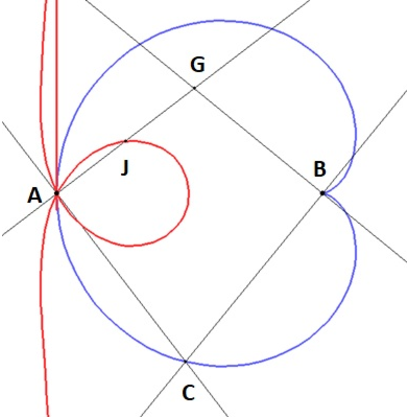
\includegraphics[height=2.0427in,keepaspectratio]{Figure3-crop.pdf}
\end{center}
 \caption{Locus of midpoints $J$ of segment $AG$ for a cardioid.}
 \label{fig13}
\end{figure}

\end{example}

When $A=(a,0)$ ($a\ne0$)and $B=(0,0)$ denote the moving point $C=(x_{0},y_{0})$,
the slopes for $CB$ and $CA$ are $k_{CB}$ $=\frac{y_{0}}{x_{0}}$ and
$k_{CA}=\frac{y_{0}}{x_{0}-a}$, respectively. The corresponding equations
for $CB$ and $CA$ are
\begin{equation}
y=-\frac{x_{0}}{y_{0}}x, \label{eq3}
\end{equation}
and
\begin{equation}
y=-\frac{\left(  x_{0}-a\right)  }{y_{0}}\left(  x-a\right), \label{eq4}
\end{equation}
respectively. The intersection of these two lines occurs when
$\frac{x_{0}}{y_{0}}x=\frac{\left(  x_{0}-a\right)  }{y_{0}}\left(  x-a\right) $.
Since $a\neq0$ we see $x=a-x_{0}$ so that $y=\left(  \frac{x_{0}}{y_{0}}\right) \left(  x_{0}-a\right)$.
In other words, the intersection is
$G=(a-x_{0},\allowbreak\left(  \frac{x_{0}}{y_{0}}\right)  \left(x_{0}-a\right)  )$
and the midpoint for $AG$ is
\[
J=\left(  X,Y\right)  =\left(  \frac{2a-x_{0}}{2},\frac{x_{0}\left(x_{0}-a\right)  }{2y_{0}}\right).
\]
But, since $C$ is a point on the cardiod $r=f(t)=1-\cos t$ we can write
$x_{0}=(1-\cos t)\cos t$ and $y_{0}=(1-\cos t)\sin t$.
Thus we obtain the following parametric equations for the locus of $J$:
\begin{align*}
X(t)  & =\frac{2a-\left(  1-\cos t\right)  \cos t}{2}\\
Y(t)  & =\frac{\left(  1-\cos t\right)  \cos t\left(  \left(  1-\cos t\right)
\cos t-a\right)  }{2\left(  1-\cos t\right)  \sin t}.
\end{align*}

\textbf{Exploration 1. }
It is not difficult to generalize this result to the problem of
identifying the locus of $J=(X,Y)$ such that $\overrightarrow{AJ}=s\overrightarrow{AG}$ for
some real number $s$.

The equation $\overrightarrow{AJ}=s\overrightarrow{AG}$ clearly defines the point $J=(X,Y)$.
The same process as used above shows that $X=a-sx_{0}$ and $Y=s\left( \frac{x_{0}}{y_{0}} \right) (x_{0}-a)$.
Since it is still the case that $\left(  x_{0},y_{0}\right)  $ is a point on the
cardioid $r=f(t)=1-\cos t$, the locus $J$ in this case is
\begin{align}
X(a,s,t)  & =a-s\left(  1-\cos t\right)  \cos t\label{cardioid}\\
Y(a,s,t)  & =\frac{s\left(  1-\cos t\right)  \cos t}{\left(  1-\cos t\right)
\sin t}\left(  \left(  1-\cos t\right)  \cos t-a\right) \nonumber
\end{align}
Figure~\ref{fig14} shows screenshots produced with Geometry Expressions \cite{GE}
of the construction when $a=-2$ and $s=0.3$, $0.7$, and $1.5$,
respectively. Maple \cite{Maple} has been used to verify that the expressions, and figures,
produced with Geometry Expressions \cite{GE} are consistent with those obtained directly
by Maple.

\textbf{Further Remarks: }
\begin{enumerate}
\item Notice that the cardioid $r=1-\cos t$ has a point of non-differentiabilty at $B=(0,0)$.
What point on the locus of $J$ corresponds to this point on the cardioid?

\item In view of the derivation in equations \ref{cardioid}, we encourage
readers to explore how the graphs varies according to the parameters $a$, $s$,
and $t$, respectively.
\end{enumerate}

\begin{figure}[htpb]
\begin{center}
\parbox[b]{1.9in}{\begin{center}
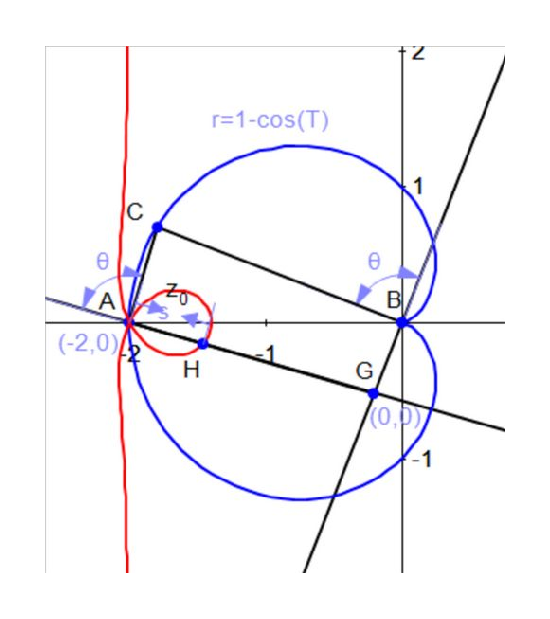
\includegraphics[height=2.0in,keepaspectratio]{PJH75I1Q.pdf}
 \\ (a)
\end{center}}
\qquad
\parbox[b]{1.7in}{\begin{center}
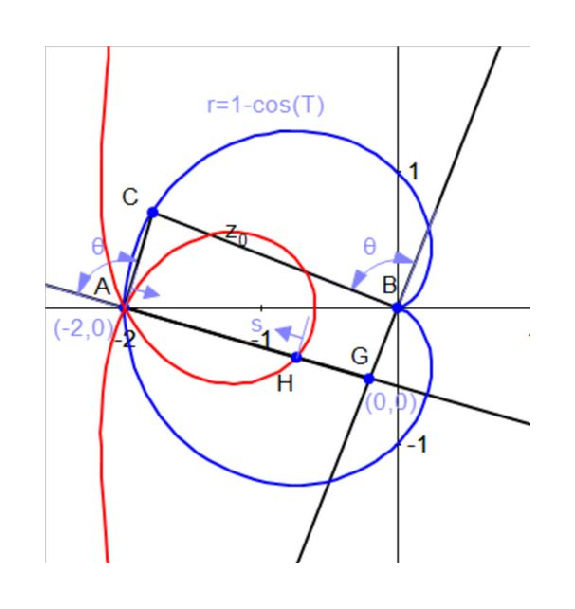
\includegraphics[height=2.0in,keepaspectratio]{PJH75I1R.pdf}
 \\ (b)
\end{center}}
\qquad
\parbox[b]{1.7in}{\begin{center}
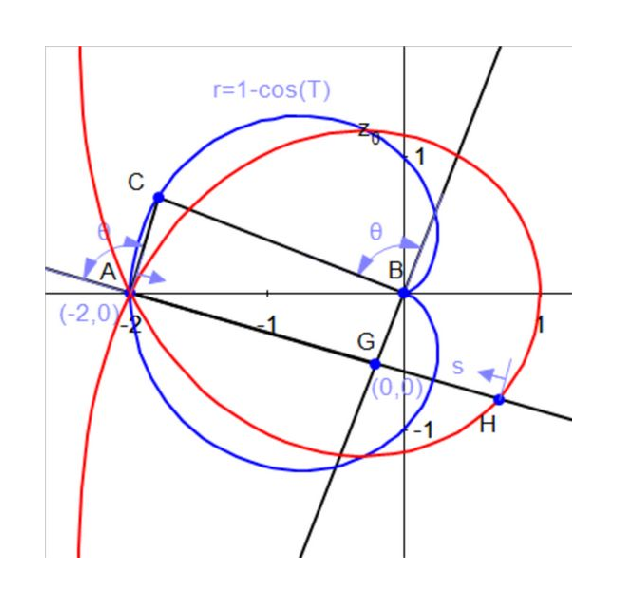
\includegraphics[height=2.0in,keepaspectratio]{PJH75I1S.pdf}
 \\ (c)
\end{center}}
\end{center}
\caption{Locus of the point $J$ (a) when $s=\frac{1}{2}$ and (b) when $s=\frac{1}{4}$.}
\label{fig14}
\end{figure}

\textbf{Exploration 2.}
To discuss the scenario when
$\measuredangle CAG = \measuredangle CBG = \pi-\theta$.
If we denote the moving point on the cardioid as $C=\left(x_{0},y_{0}\right)$
and the intersection of lines $BG$ and $AG$ as $G=\left(  x,y\right)$.
The slopes for $CB$ and $CA$ are $k_{CB} = \frac{y_{0}}{x_{0}}$
and $k_{CA}=\frac{y_{0}}{x_{0}-a}$, respectively, so that
$\theta_{1}=\arctan\left(  \frac{y_{0}}{x_{0}}\right)$ and
$\theta_{2}=\arctan\left(  \frac{y_{0}}{x_{0}-a}\right)$.
The equations for $BG$ and $AG$ can be written as
\begin{equation}
y=\tan\left(  \theta_{1}-\theta\right)  x \label{eq7}
\end{equation}
and
\begin{equation}
y=\tan\left(  \theta_{2}+\theta\right)  \left(  x-a\right).  \label{eq8}
\end{equation}
When Maple \cite{Maple} solves equations (\ref{eq7}) and (\ref{eq8}) it produces
\[
x=\frac{a\tan\left(  -\arctan\left(  \frac{y_{0}}{-x_{0}+a}\right)
+\theta\right)  }{\tan\left(  -\arctan\left(  \frac{y_{0}}{-x_{0}+a}\right)
+\theta\right)  +\tan\left(  -\arctan\left(  \frac{y_{0}}{x_{0}}\right)
+\theta\right)  }.
\]
Then, using equation (\ref{eq5}) or (\ref{eq6}) to find $y$, the result is too long
to display but can be found in the supplemental resource [S5].
More explorations can be found in supplemental resources [S8] and [S11].
Continuing, we substitute $x_{0}=\left(  1-\cos t\right)  \cos t$ and
$y_{0}=\left(  1-\cos t\right)  \sin t$ into the expressions for $x$ and $y$ to find
the intersection between $AG$ and $BG$, which we denote it as $G=(x,y)$. Since
the locus $J=(X,Y)$ is such that $\overrightarrow{AJ}=s\overrightarrow{AG}$
for some real number $s$, the locus of the points $J=(X_1,Y_1)$ is found to satisfy
\[
\left[
\begin{array}
[c]{c}%
X_{1}\left(  a,s,t,\theta\right) \\
Y_{1}\left(  a,s,t,\theta\right)
\end{array}
\right]  =\left[
\begin{array}
[c]{c}%
s\left(  x\left(  a,s,t,\theta\right)  -a\right) \\
sy\left(  a,s,t,\theta\right)
\end{array}
\right]  =s\left[
\begin{array}
[c]{c}%
x\left(  a,s,t,\theta\right)  -a\\
y\left(  a,s,t,\theta\right)
\end{array}
\right]  +\left[
\begin{array}
[c]{c}%
a\\
0
\end{array}
\right]  .
\]
The final expressions obtained by Maple \cite{Maple} for
$X_{1}\left(  a,s,t,\theta\right)$ and $Y_{1}\left(a,s,t,\theta\right)$
are shown in the following screenshots:
\begin{align*}
&
%TCIMACRO{\FRAME{itbpF}{6.5628in}{0.8036in}{0in}{}{}{Figure}%
%{\special{ language "Scientific Word";  type "GRAPHIC";
%maintain-aspect-ratio TRUE;  display "USEDEF";  valid_file "T";
%width 6.5628in;  height 0.8036in;  depth 0in;  original-width 6.6595in;
%original-height 0.7903in;  cropleft "0";  croptop "1";  cropright "1";
%cropbottom "0";  tempfilename 'PJH75I1T.wmf';tempfile-properties "XPR";}} }%
%BeginExpansion
{
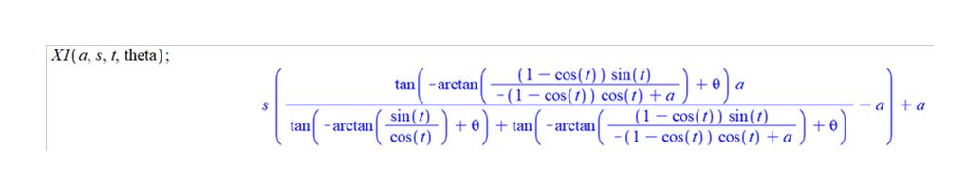
\includegraphics[width=\textwidth,keepaspectratio]{PJH75I1T.pdf}
}
%EndExpansion
\\
&
%TCIMACRO{\FRAME{itbpF}{6.5628in}{0.9296in}{0in}{}{}{Figure}%
%{\special{ language "Scientific Word";  type "GRAPHIC";
%maintain-aspect-ratio TRUE;  display "USEDEF";  valid_file "T";
%width 6.5628in;  height 0.9296in;  depth 0in;  original-width 6.6595in;
%original-height 0.9189in;  cropleft "0";  croptop "1";  cropright "1";
%cropbottom "0";  tempfilename 'PJH75I1U.wmf';tempfile-properties "XPR";}} }%
%BeginExpansion
{
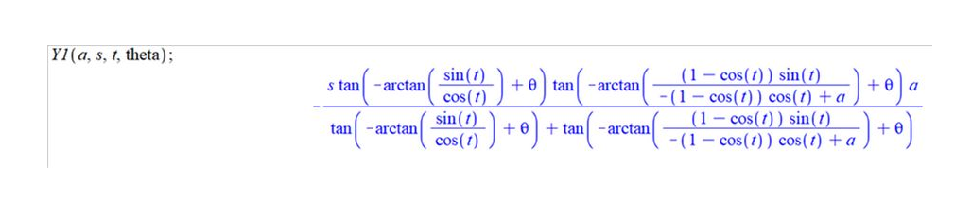
\includegraphics[width=\textwidth,keepaspectratio]{PJH75I1U.pdf}
}
%EndExpansion
\end{align*}

The corresponding parametric equations for the locus of $J$ obtained 
from Geometry Expressions \cite{GE} is, when converted into the Maple
syntax:
\[%
%TCIMACRO{\FRAME{itbpF}{6.5628in}{0.895in}{0in}{}{}{Figure}%
%{\special{ language "Scientific Word";  type "GRAPHIC";
%maintain-aspect-ratio TRUE;  display "USEDEF";  valid_file "T";
%width 6.5628in;  height 0.895in;  depth 0in;  original-width 6.6595in;
%original-height 0.8834in;  cropleft "0";  croptop "1";  cropright "1";
%cropbottom "0";  tempfilename 'PJH75I1V.wmf';tempfile-properties "XPR";}} }%
%BeginExpansion
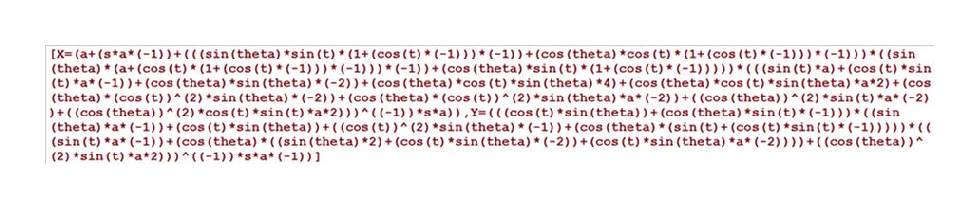
\includegraphics[width=\textwidth,keepaspectratio]{PJH75I1V.pdf}
%EndExpansion
\]

Supplemental resources [S5], [S8] and [S11] show that the family of locus plots
for the parametric equations $[X_{1}(-2,s,t,\theta),Y_{1}(-2,s,t,\theta]$
obtained from Maple \cite{Maple} are identical to $[X(-2,s,t,\theta),Y(-2,s,t,\theta)]$
obtained from Geometry Expressions \cite{GE}.
For the specific situation when $a=-2$, $s=0.7$, and $\theta=\frac{2\pi}{3}$,
Figure~\ref{fig15} shows locus produced by Maple with blue diamonds and
the locus produced by Geometry Expressions with red crosses (and the
original cardioid in cyan). The actual proof that the two representations are
equivalent is not difficult, but it is tedious and the final expressions are not
immediately illuminating, so these details are omitted here.
 
\begin{figure}[htpb]
\begin{center}
 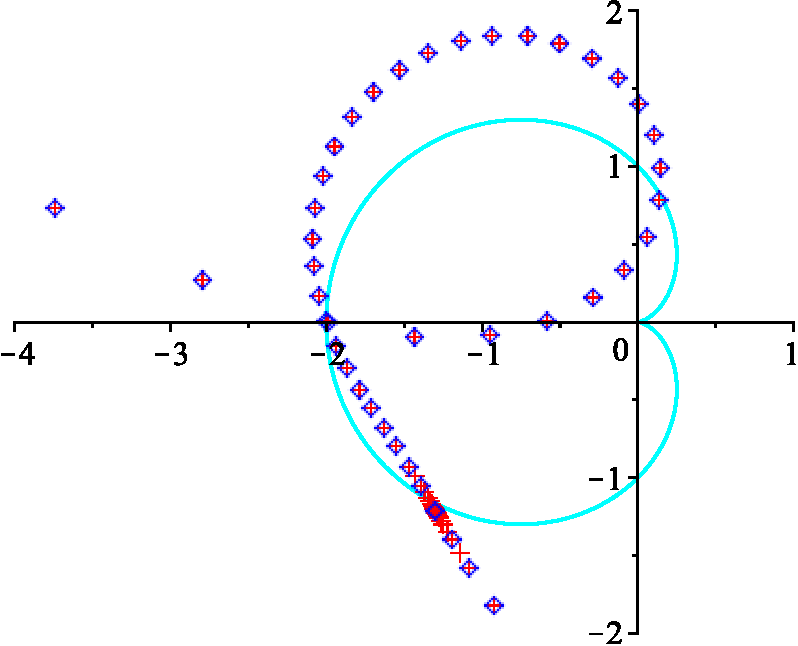
\includegraphics[height=2.3in,keepaspectratio]{PJH75I1Z-crop.pdf}
\end{center}
\caption{Comparison of the parametric curves
              $\left[X_1\left(-2,0.7,t,\frac{2\pi}{3}\right), Y_1\left(-2,0.7,t,\frac{2\pi}{3}\right)\right]$
               from Maple (in blue diamonds) and 
              $\left[X\left(-2,0.7,t,\frac{2\pi}{3}\right), Y\left(-2,0.7,t,\frac{2\pi}{3}\right)\right]$,
               from Geometry Expressions (in red crosses).}
\label{fig15}
\end{figure}

\section{Conclusion} \label{conc}

It is clear that technological tools provide us with many crucial intuitions
before we attempt more rigorous analytical solutions. Here we have gained
geometric intuitions while using a DGS such as \cite{CP} or \cite{GE}.
We also showed the utility of a CAS, such as Maple \cite{Maple}, for verifying that our
analytical solutions are consistent with our initial intuitions. The
complexity level of the problems we posed vary from the simple to the
difficult. Many of our solutions are accessible to students from high school.
Others require more advanced mathematics often taught in universities.
The more advanced problems
are excellent examples for future teachers to explore and to understand before they
try to explain the simpler problems to their students.

Evolving technological tools definitely have made mathematics fun and
accessible. They also allow the exploration of more
challenging and theoretical mathematics. We hope that when mathematics is made
more accessible to students, more students will be inspired to
investigate problems ranging from the simple to the more challenging, and even open questions.
We do not expect that exam-oriented curricula will change in the short term.
However, encouraging a greater interest in mathematics for students, and in
particular providing them with the technological tools to solve challenging
and intricate problems beyond the reach of pencil-and-paper, is an important
step for cultivating creativity and innovation.

\section{Acknowledgements} \label{ack}

The authors would like to thank Dao Hoang and Phil Todd
(creator of Geometry Expressions \cite{GE})
for providing the illuminating dynamic figures 
(see supplemental resources [S6]--[S11]). The authors also would like to thank Qiuxia Li for providing the
proofs of some examples and numerous inspiring discussions about the level of
high school math content knowledge from her teaching experiences in China.

\section{Supplementary Electronic Materials}

\begin{center}
 \begin{tabular}{|c|c|c|c|} \hline
   Content & Maple & Geometry Expressions & HTML \\ \hline
   Section 2.2 & [S1] & --- & --- \\
   Section 3.1 & [S2] & [S6] & [S9] \\
   Exercise 6  & [S3] & ---    & --- \\
   Example 7  & [S4] & [S7] & [S10] \\
   Example 8  & [S5] & [S8] & [S11] \\ \hline
 \end{tabular}
\end{center}

\begin{thebibliography}{9}                                                                                                %
\bibitem {ATCM2018}Yang, W.C. (2018) Strong Algebraic Manipulation Skills Are
Not Adequate For Cultivating Creativity And Innovation, \textit{Proceedings of
the ATCM 2018}, November 20-24, ISBN 978-0-9972807-2-2, 2018.

\bibitem {CP}ClassPad Manager, a product of CASIO, \url{https://edu.casio.com/freetrial/freetrial\_list.php}.

\bibitem {GE}Geometry Expressions, see \url{http://www.geometryexpressions.com/}.

\bibitem {GI}Geometry Interactive Mathematical Arts (GInMA): A Dynamic
Geometry System, see \url{http://deoma-cmd.ru/en/Products/Geometry/GInMA.aspx}.

\bibitem {June2017}Yang, W.-C., (2017) From Static Locus Problems to Exploring
Mathematics with Technological Tools, \textit{The Electronic Journal of
Mathematics and Technology}, Volume 11, Number 2, pp. 67-88, 2017.

\bibitem {Maple}Maple, A product of Maplesoft, see \url{http://Maplesoft.com/}.

\bibitem {MacandYang}McAndrew, A., Yang, W.-C. (2016). Locus and Optimization
Problems in Lower and Higher Dimensions. The Electronic Journal of Mathematics
and Technology, 10(2), 69-83,
\url{https://php.radford.edu/~ejmt/deliveryBoy.php?paper=eJMT\_v10n2p1}.

\bibitem {Gao}Shi Gi Gin Bang. \textquotedblleft Strategies for High School
Mathematics Complete Review\textquotedblright. In: ed. by Cuiun Guan Zhiming.
Century Gold. Yanbian University Press, 2015.

\bibitem {YangandS}Yang, W.-C., and Shelomovskii,V. 2D and 3D Loci Inspired by
an Entrance Problem and Technologies, \textit{The Electronic Journal of
Mathematics and Technology}, Volume 11, Number 3, pp. 194-208, 2017.
\end{thebibliography}


\end{document}
